\documentclass[./dissertation.tex]{subfiles}
\begin{document}
\part{Introduction}
\chapter{Background}
\label{chap:fond}

\begin{minipage}{12cm}\textit{Semiconductor devices and integrated circuits are nowadays operated in a number of hostile environments, therefore it worth to analyze all of them in order to determine what threat show up. Moreover in this chapter it will shown the most common effects on MOSFET based devices as well as the possible architectural solution of the state of the art}

\end{minipage}

\vspace{1.30cm}
\begin{center}
    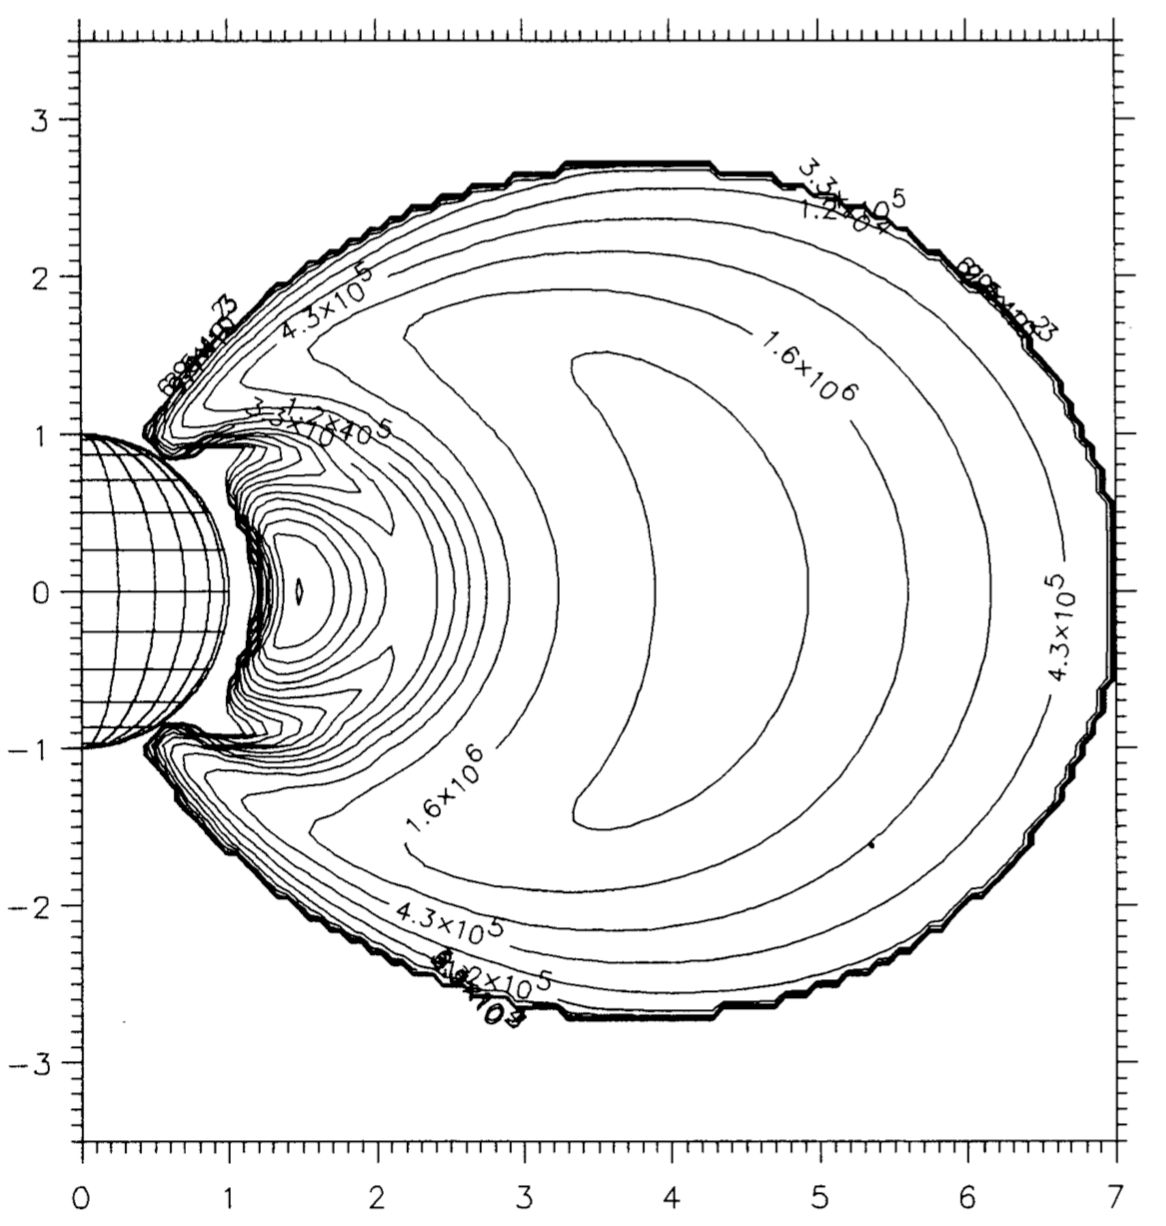
\includegraphics[scale=0.40]{Figures/radiation.png}
\end{center}
\vspace*{1cm}
\newpage

\section{The Space Environment}
The Earth and its immediate surroundings are protected by the atmosphere, which acts as a semi-permeable shield letting through light and heat while stopping radiation and UV's; because no such protection is available in space, human beings and electronics (onboard Earth orbiting satellites, space shuttles, space probes) must be able to cope with the resulting set of constraints. Based on several tens  of years of this  space  era, a detailed analysis of the problems on satellites shows that the part due to the radiation  environment  is  significant. It appears  that  the malfunctions   are   due to problems   linked to the   space environment (9 to 21\%), electronic  problems (6 to 16\%), design  problems (1 1  to 25\%), quality  problems  (1 to 8\%), other   problems (11  to   33\%) and  problems   that are still unexplained (19 to  53\%) \cite{bib2}.  It is clear  that the unexplained problems  are either problems  linked to the space environment, to the electronics, to   the design, or otherwise   but   the information  collected  on  the  ground is generally not sufficient to define the origin  of  the  problem. The space environment is largely  responsible   for   about 20\% of the anomalies  occurring  on  satellites  and a  better  knowledge of that  environment  could  only  increase  the  average lifetime of space vehicles.

So the study of the space environment and its causes started, in all its great variety of environments depending on different orbital levels and electromagnetic forces involved. The  degradation  and  disturbances induced by space radiation in the materials  and the  electronic  components are phenomena that  have  been  studied for many  years.\cite{bib2} It resulted in a basic classification of damages, either for Humans and for Electronics that can be easily divided into two groups each:

For Electronics
\begin{enumerate}
    \item \textbf{Cumulative}  such  as the degradation  of thermal control coatings, optics  and  electronics  and  the  erosion  of materials;
    \item \textbf{Sporadic}  such as noises in the  detectors  and optics,   single  event  effects in highly  integrated  electronic circuits and electrostatic discharges.
\end{enumerate}

while for humans

\begin{enumerate}
    \item \textbf{Immediate}, permanent or delayed  non  stochastic  effects (destruction or modification of cells), the speed with which the symptoms appear  and  their  seriousness  increase in proportion to the exposure to the radiation;
    \item \textbf {Stochastic}   associated  with the modifications to the cells whose probability of appearing in the long term  increases in proportion to  the irradiation  (cancers,  leukemia, (SET) Program. genetic effects).
\end{enumerate}

\subsection{Solar Activity}
Sun is either a source and modulator of space radiation, its activity can be described using a cyclical model. Each cycle has approximately is 11 years long. In this time span the Sun has 7 years of maximum activity and 4 at its minimum, the transition is considered sharp even though it is indeed continuous. Moreover every 11 years cycle the Sun reverse its magnetic polarity, this leads to an actual 22 years period between two equal configurations.

Usually two main indicators are used to describe the solar activity:
\begin{enumerate}
    \item F10.7 - 10.7 cm radiation flux
    \item Sunspots count - The numbering of sunspot
cycles began in 1749 and it is currently near the end of solar
cycle 23. The record of F10.7 began part way through solar
cycle 18 in the year 1947
\end{enumerate}

\begin{figure}[h!]
\centering
  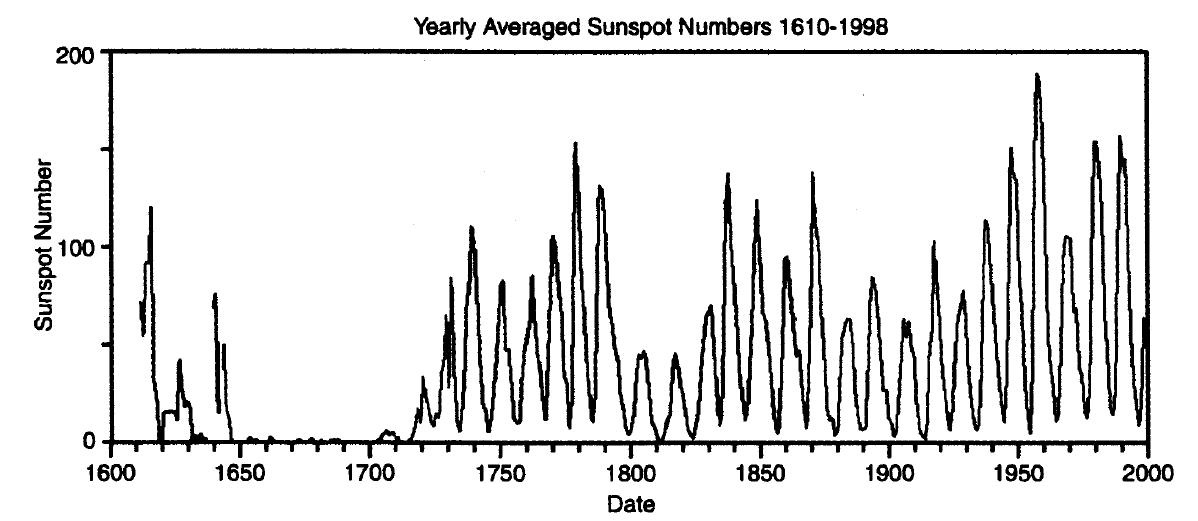
\includegraphics[scale = 0.50]{imgs/sunspot.PNG}
  \caption{The observed record of yearly averaged sunspot numbers \cite{bib2}}
  \label{fig:magnetosphere}
\end{figure}
\begin{figure}[h!]
\centering
  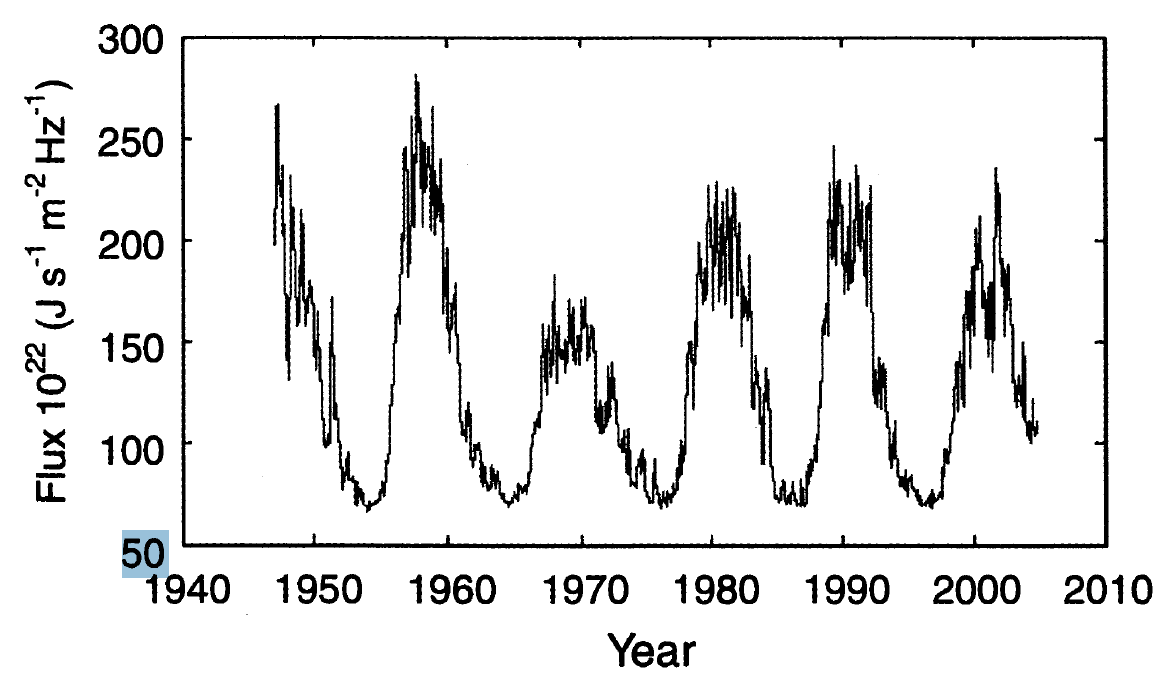
\includegraphics[scale = 0.50]{imgs/F10sun.PNG}
  \caption{Measured values of solar 10.7 cm radio flux \cite{bib2}}
  \label{fig:magnetosphere}
\end{figure}

Large solar particle events  are known to occur  with greater    frequency   during   the    declining   phase of solar maximum [3]. Trapped  electron  fluxes  also  tend to be  higher during the declining  phase [4]. Trapped proton  fluxes in  low earth  orbit (LEO) reach their  maximum during solar minimum but exactly when this peak is reached depends on the particular location [5]. Galactic cosmic ray fluxes are also at a maximum during  solar minimum but  in addition  depend  on the magnetic polarity of the sun [6]. 

\newpage

\subsection{Cosmic Rays}
With Galactic Cosmic Rays (GCR) it is intended all those highly-charged particles that have been generated outside our solar system, even thought their precise origin  is unknown, scientific community believes that Supernovas explosions may be the first source. Some general characteristics of GCR are listed in the following table

% Please add the following required packages to your document preamble:
\begin{table}[h!]
\begin{tabular}{@{}lllll@{}}
\toprule
Hadron Composition                                                                    & Energy                           & Flux                                                         & Radiation Effects & Metric \\ \midrule
\begin{tabular}[c]{@{}l@{}}87\% Protons\\ 12\% Alpha\\ 1\% Heavy Ions\end{tabular} & up to 10\textasciicircum{}11 GeV & 1 to 10 cm\textasciicircum{}\{-2\} s\textasciicircum{}\{-1\} & SEE               & LET    \\ \bottomrule
\end{tabular}
\end{table}
But it is possible to have a deeper look at the relative abundances in \ref{Fig:abun}.


\begin{figure}[!ht]
   \centering
    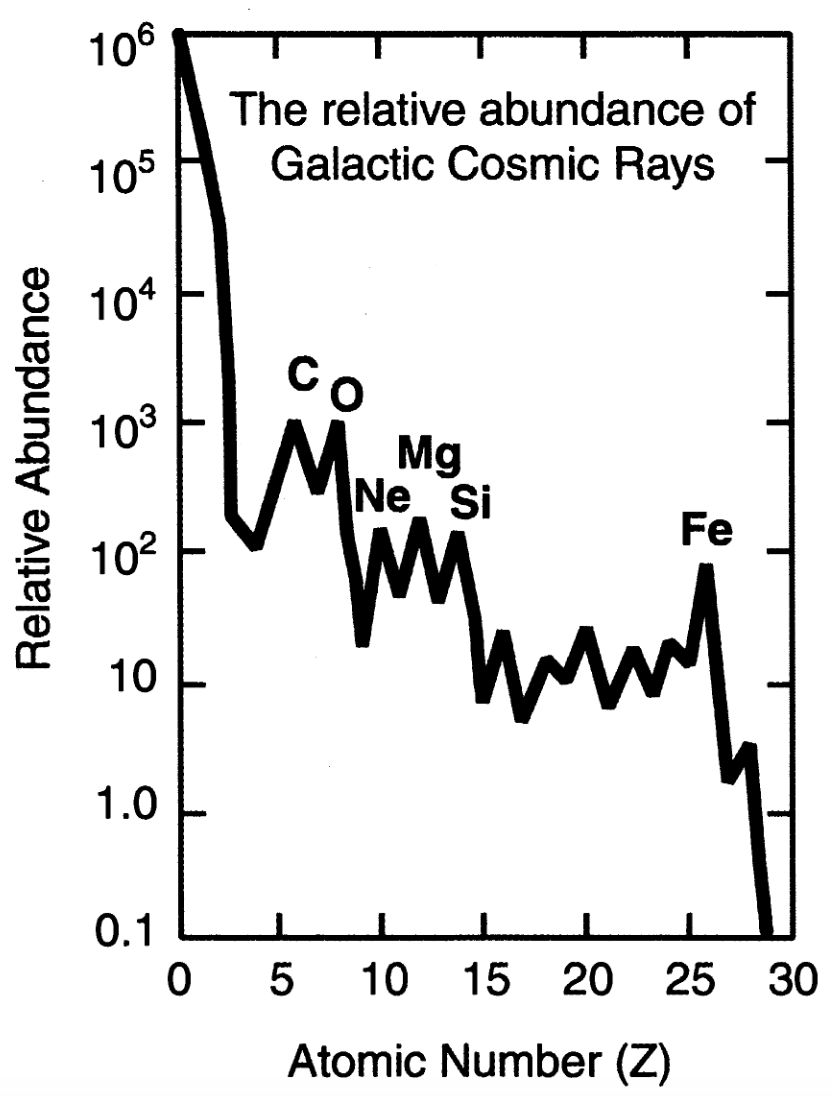
\includegraphics[scale=.5]{imgs/Abundances.png}
   \caption{Abundances of GCR up through Z = 28}
   \label{Fig:abun}
\end{figure}

All the elements in the Periodic Table up to Uranium are present in GCR although there is a steep drop-off for atomic numbers higher than iron (Z=26). Their source isn't the only unknown feature of GCR. We saw that they can reach energies up to $10^{11}GeV$, but the causes behind such acceleration are still to be comprehended. On the other hand their flux is really small, limited to a few $cm^{-2}s^{-1}$. Typical GCR energies and fluxes are shown in Fig. \ref{fig:enflux}.


\begin{figure}[!ht]
   \centering
    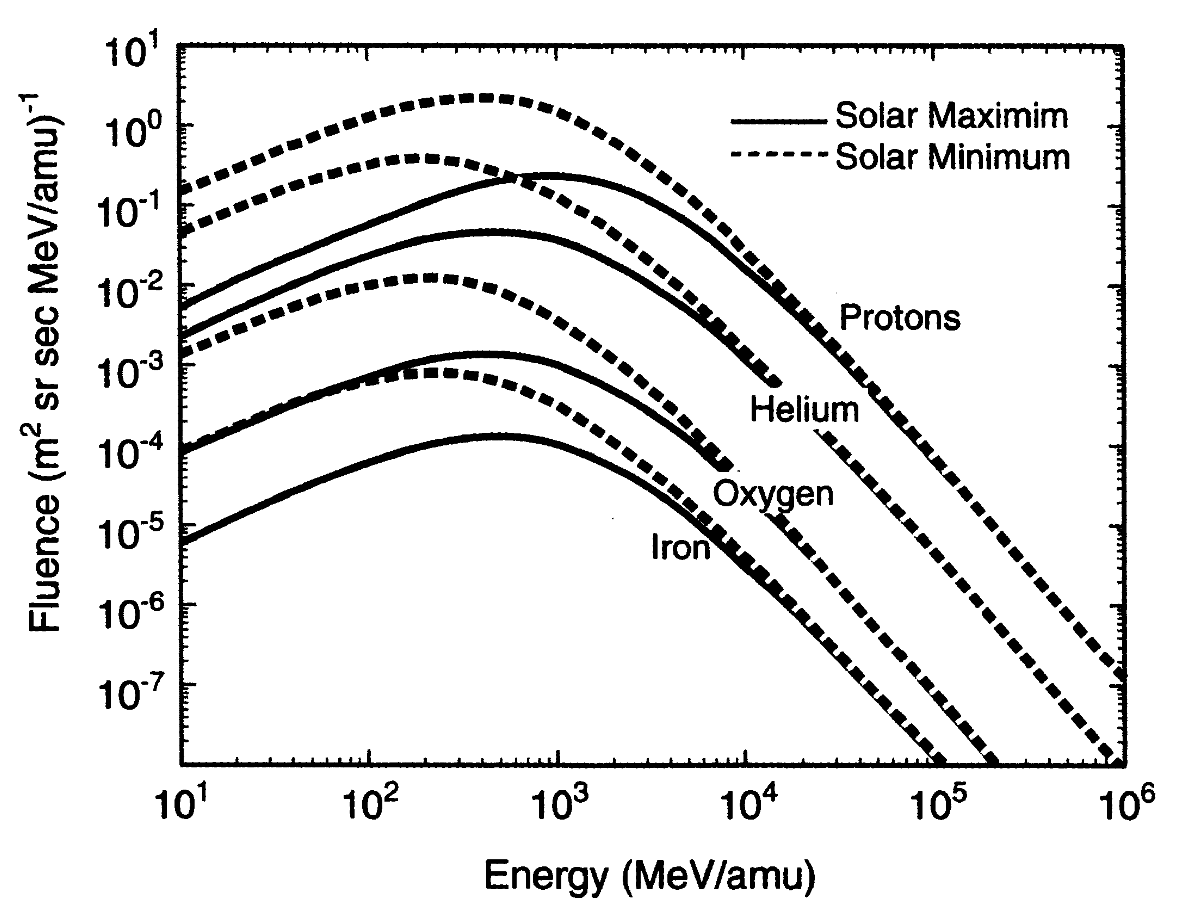
\includegraphics[scale=.5]{imgs/GCR_energy_p.png}
   \caption{GCR energy spectra for protons, helium, oxygen and iron during solar maximum and solar minimum conditions}
   \label{fig:enflux}
\end{figure}
The peak around $1GeV$ is due to the moderation effect of the solar wind and solar magnetic field, still another expansion for the inverse proportionality of GCR Flux and solar activity.
\begin{figure}[!h]
   \centering
    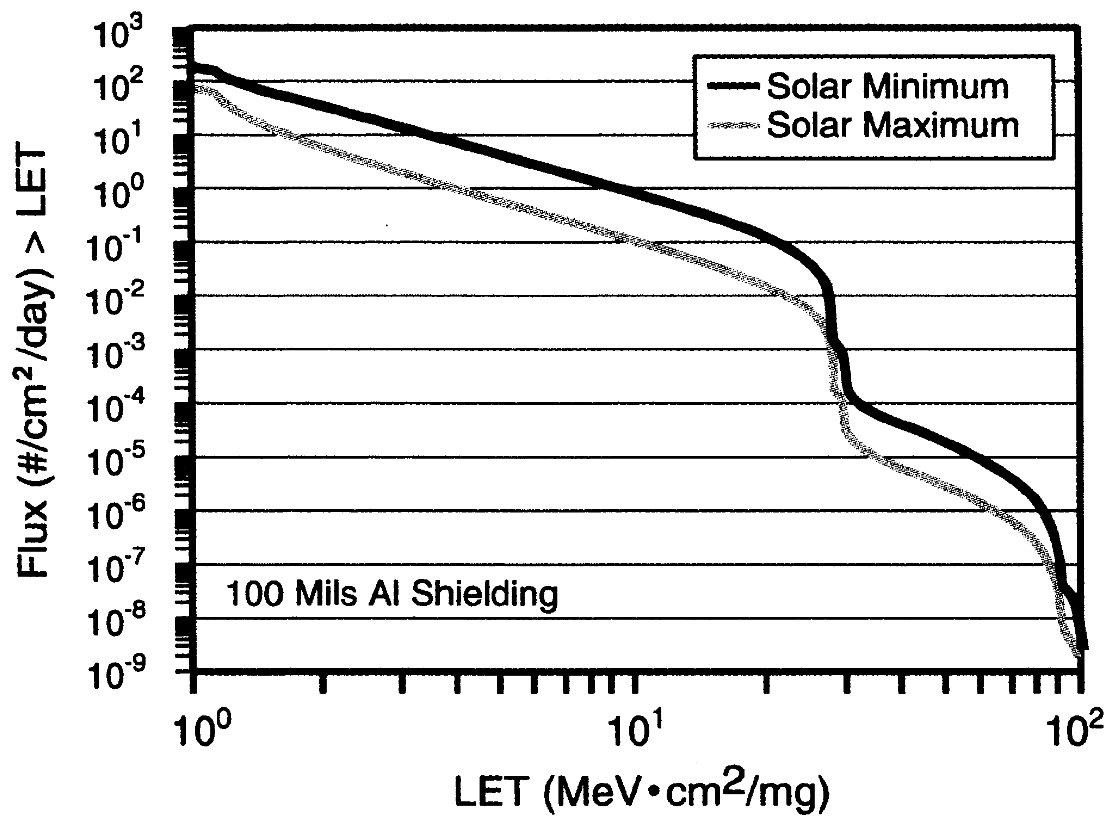
\includegraphics[scale=.5]{imgs/LET_sun.png}
   \caption{Integral LET spectra  for GCR during  solar  maximum  and solar minimum}
   \label{fig:sub1}
\end{figure}
Speaking about the Radiation Effects that these GCR can cause, the main Result of impact is a Single Event Effects (SEE) and the metric to usually utilized to describe the heavy ion induced SEE is the Linear Energy Transfer (LET) which can be defined as the energy lost by the ionizing particle per unit of path length in the sensitive section of the device. So it is possible to convert Fig. \ref{fig:enflux} into the spectrum per LET, integrating we can see the difference between the minimum and maximum activity level of the Sun. In the following image all the contributes from all the elements, starting from protons up to uranium, have been considered. The ordinate gives the Flux of particles having a LET above the corresponding abscissa. 

The LET Metric can be applied in GEO and Interplanetary missions, in absence of geomagnetic attenuation. For instance, due to basic interaction between charged particles and Earth magnetic field they tend to follow the geomagnetic lines and so parallel to the plant surface at the equator. Thus the energy is mostly deflected away. The Effect of the Geomagnetic field on the incident GCR-LET spectrum during solar minimum is discussed for various orbits in [12]


\subsection{Radiation Belts}
Earth is relatively well protected against external influences such as radiation coming from outer space. In these terms we can imagine the Earth Magnetosphere as the natural cavity in the interplanetary medium that serve to the cause. It is compressed on the solar side and highly extended on the anti-solar side. Poles represent the only space offered to the interplanetary particles to penetrate into the upper atmosphere. Meanwhile the charged particles close to Earth can be trapped by the magnetic field and form the Radiation Belts. As shown in Fig: \ref{fig:magnetosphere} the radiation belts only occupy a limited internal region of the whole magnetosphere. Starting from the closest section to Earth it's possible to identify the upper atmosphere, constant over time. On the opposite end, we cannot really define a boundary due to its strong dependence on solar wind and magnetic field.

\begin{figure}[h!]
\centering
  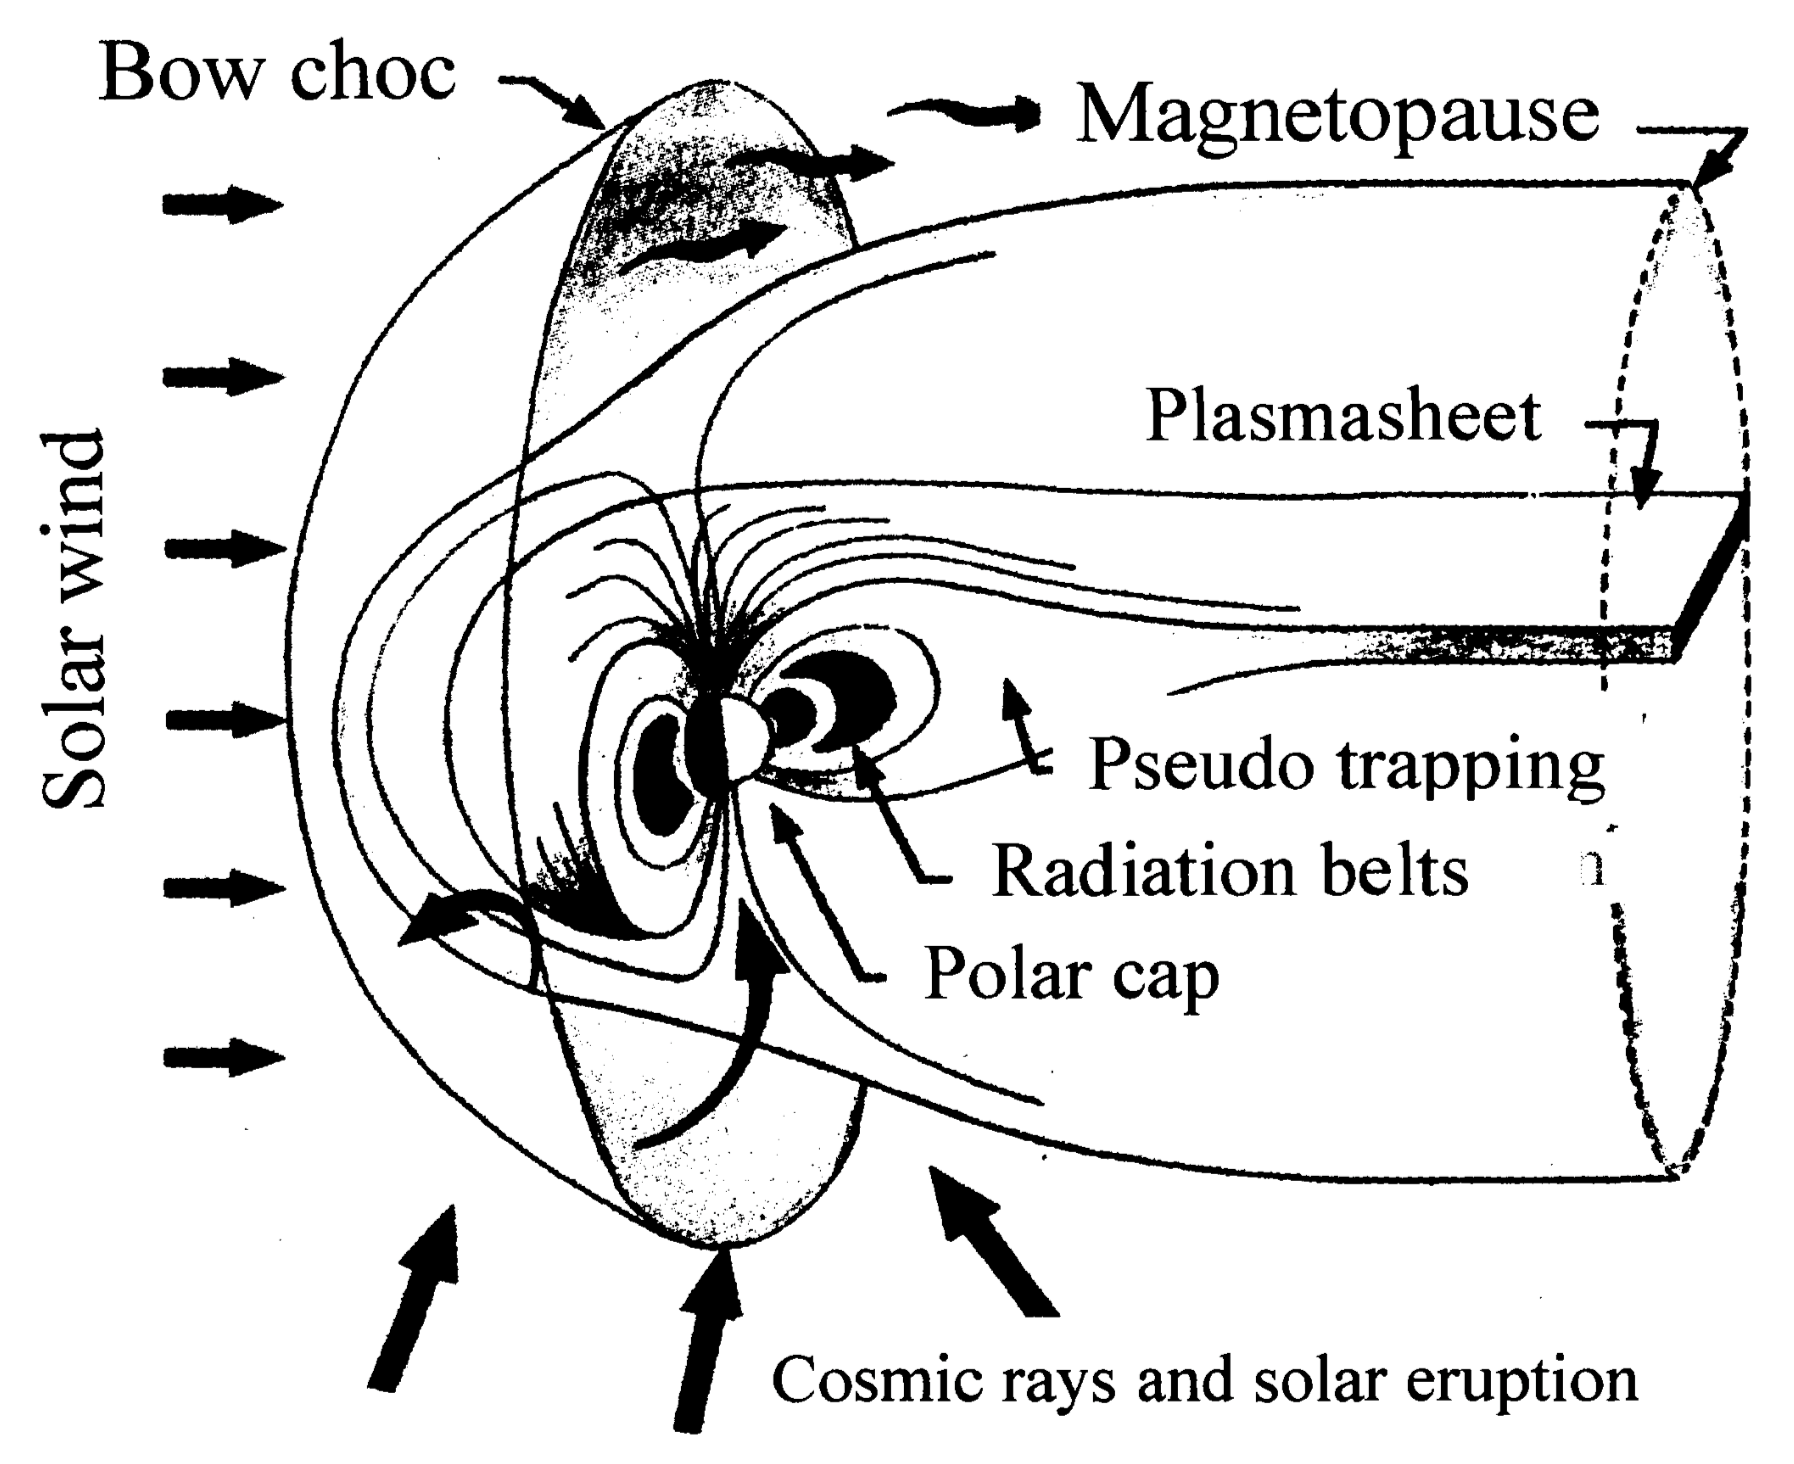
\includegraphics[scale = 0.30]{Figures/magnetosphere.png}
  \caption{Magnetosphere with respect to Radiation Belts \cite{bib2}}
  \label{fig:magnetosphere}
\end{figure}

In the Earth Magnetosphere we can define the magnetic field as the sum of two contributes:
\begin{enumerate}
    \item \textbf{Main Component} - This term is based on the convection motion in the core of the planet
    \item \textbf{External Origin} - This includes all the permanent magnets of the terrestrial crust.
\end{enumerate}

In a zero order approximation the field can be considered bipolar. However it is way more accurate to take an off-centered and tilted dipolar magnetic field as approximation. This gives us a Dipole not centered in the center of Earth and having its axis not parallel to the earth one. This geometry leads to an anomaly in the magnetic field, a region in which the  field is weaker, called the South Atlantic Anomaly, as shown in Fig. \ref{fig:radbel1}. It is important to observe that the magnetic field on Earth is evolving on a long term basis (secular drift), in particular the South Atlantic Anomaly, which is drifting south-eastwards. As the present time we note:
\begin{itemize}
    \item a decrease in the intensity of $27\frac{nT}{year}$ (0.05 \% a year) \cite{bib2}
    \item a drift of the axis, resulting in a westward rotation of the
southern end of the dipole (0.014$\deg$ a year) and an increase in
the shift towards the West Pacific close to 3 km a year. \cite{bib2}
\end{itemize}



\begin{figure}[h!]
\centering
  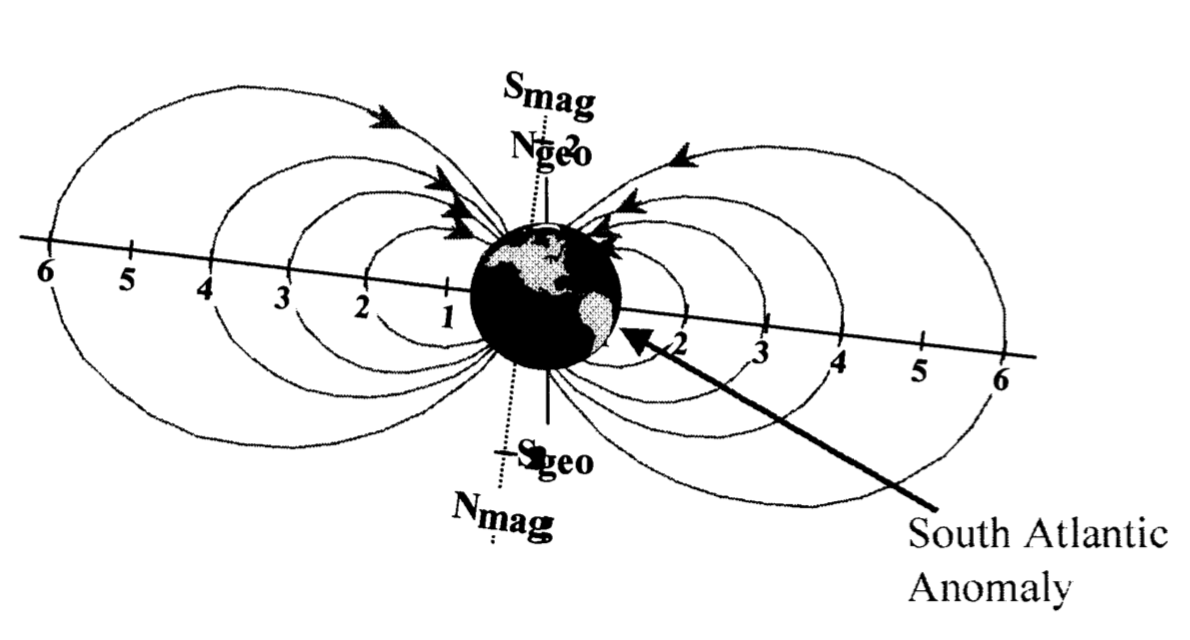
\includegraphics[scale = 0.50]{imgs/radbelt1.png}
  \caption{Dipolar magnetic field tilted and off-center with respect to Earth. \cite{bib2}}
  \label{fig:radbel1}
\end{figure}

\paragraph{Dynamics of the charged particles}

In order to better understand and describe the dynamics of the charged particle in the magnetosphere, we can define a reference system and its coordinates. 
\begin{itemize}
    \item $r$ is the distance from the center of the dipole
    \item $\lambda$ is the latitude with $\theta$ its colatitude ($\theta = \frac{\pi}{2} - \lambda$)
    \item $\phi$ its magnetic longitude
\end{itemize}

Last we need to describe the Field lines or force line by the McIlwain parameter L, roughly equal to the distance from the center of the planet to the intersection point of that force line with the magnetic equatorial plane. So a single point in the field is called B, modulus of the magnetic field.

All charged particles subject to an electromagnetic field will be subject to the Lorentz force 
\begin{equation}
    F = q (v \wedge B + E )
\end{equation}

Under these conditions, the movement of the high-energy particles can be generally broken down into three basic periodic movements.
\paragraph{Gyration}
All the charged particles in a magnetic field will rotate around the line of field. This is called Gyration and we can define this movement 
\begin{enumerate}
    \item the Larmor radius $r_L = \frac{mv^2}{qB}$ 
    \item the relativistic magnetic moment $\mu = \frac{mv^2}{2B}$
\end{enumerate}


\paragraph{Bounce}
If a particle only has a component of its velocity parallel to the magnetic field, then it will move along the field lines. In their motion they keep the magnetic moment $\mu$ constant. Since the magnetic moment has to stay constant, while moving from the equator towards the poles, it is possible to notice a strongly increasing magnetic field. It is necessary that the
perpendicular component of the speed should increase in order
for p to remain constant.\cite{bib2}

\paragraph{Drift}
in order to simplify the problem, we place ourselves on the magnetic equator. Since the magnetic field of the planets has a radial gradient, the gyration cannot take place in a constant Larmor radius. Indeed, the magnetic field along a gyration becomes stronger if the particle approaches the planet, the Larmor radius is then smaller and therefore the radius of the trajectory's curve is also smaller. The particle will thus be able to move away from the planet, the magnetic field will be weaker and therefore the Larmor radius and the radius of the trajectory's curve will be greater. The particle therefore does not go through a simple circle but along a more complex trajectory. This movement breaks down into a simple gyration (circular) and a rotation movement around the planet: this is the drift movement.

\begin{figure}[h!]
\centering
  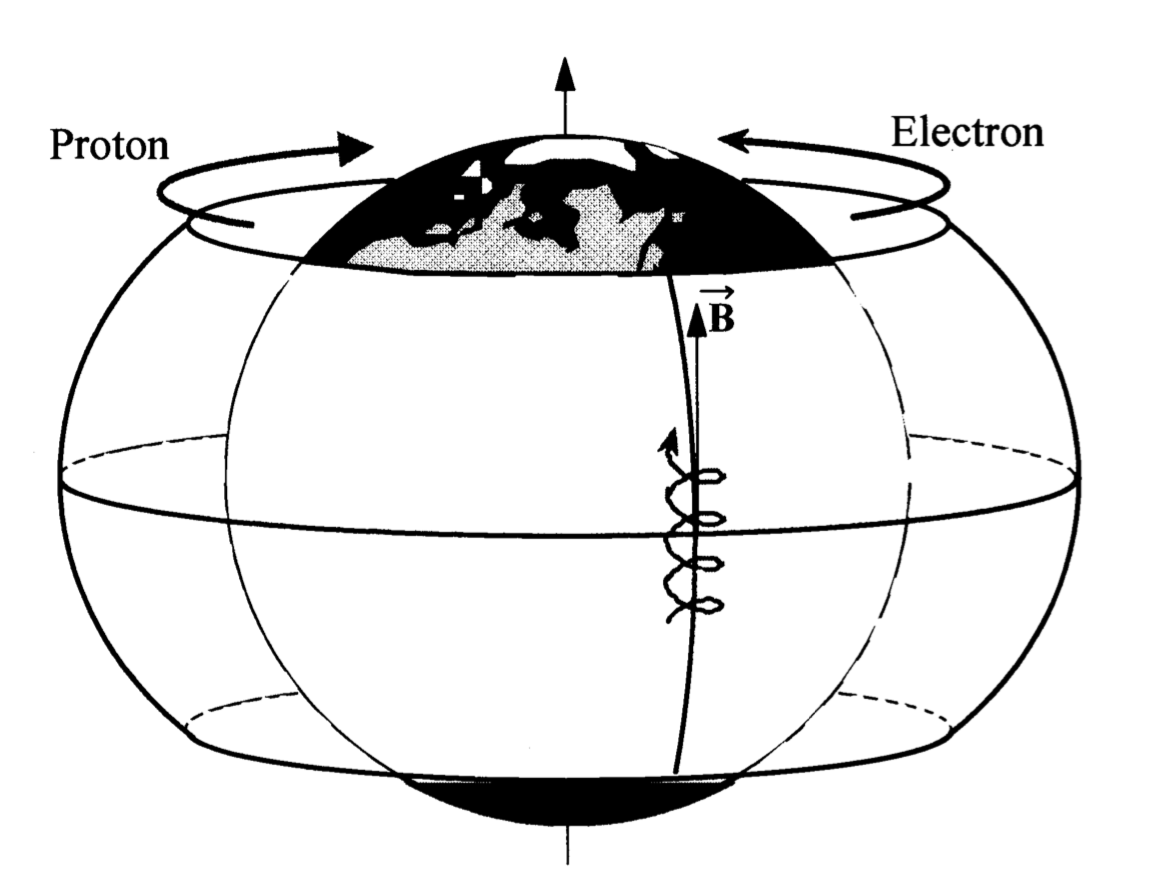
\includegraphics[scale = 0.50]{imgs/radbelt2.png}
  \caption{Composition of a charged particle's three periodic movements: gyration, bounce and drift. The particle then follows a torus surface called a drift shell. \cite{bib2}}
  \label{fig:radbel2}
\end{figure}

A charged particle submitted to these three basic [81] and
periodic movements then moves through torus shaped surfaces
around the Earth, which are commonly called drift shells Fig \ref{fig:radbel2}. The periods associated with each of these basic
movements for a 3 MeV electron at L=3 are respectively $2.14 10^{-4}$
s, 0.19 s and 504 s. The disparity between the periods is
very great, a factor of the order of 1000 should be noted
between each of them going from the gyration movement to
the drift movement.

Due to the magnetic field in proximity of Earth make all the relativistic charged particles to remain trapped in a quasi periodic movement. These conditions are perfect to start an increasing high energy charged particles enables, creating the so called radiation Belts.
Given the previously presented trajectories, the Radiation Belts assume a toroidal shape surrounding the Earth. The atmosphere is the lower bound while the outer limit is not well defined and may be time variable.

During the first space missions, J. Van Allen has discovered that mostly all the trapped particles are Protons and Electrons, having an Energy range between come KeV and hundreds of MeV. Below there is a representation of the Proton belt (Fig.\ref{fig:radbel3}), pretty stable and constant in time, with energies from some MeV to hundreds of MeV.

On the other hand, the electron belt is more complex (Fig. \ref{fig:radbel4}) and has two
maximums respectively corresponding to the internal and
external zones:
- the first one centered on L = 1.4 extends up to L = 2.8; the
electron populations are relatively stable there and can reach
maximum energy levels of the order of 10 or even 30 MeV;
- the second one, centered on L = 5, extends from L = 2.8 to
L = 10; the electron flows there are much more variable and
the energy levels can be as high as 7 MeV.

\begin{figure}[h!]
\centering
  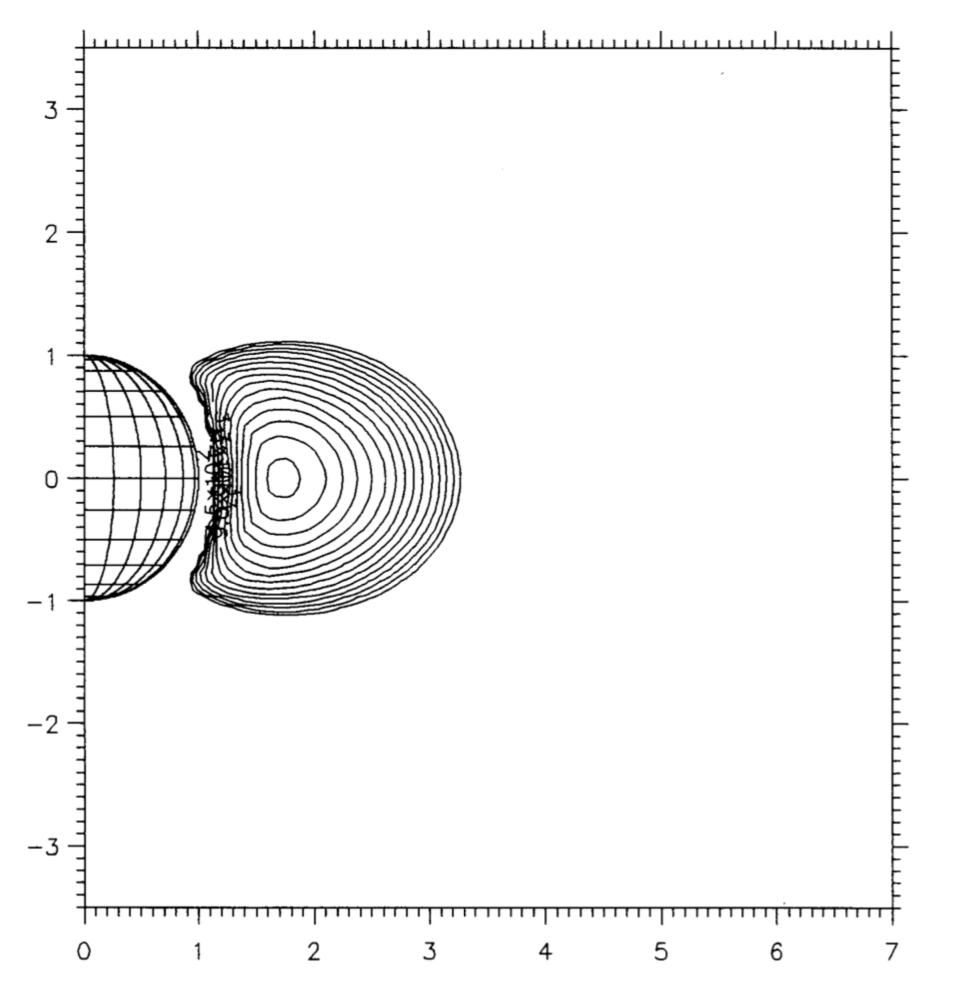
\includegraphics[scale = 0.50]{imgs/radbelt3.png}
  \caption{Proton radiation belt \cite{bib2}}
  \label{fig:radbel3}
\end{figure}

\begin{figure}[h!]
\centering
  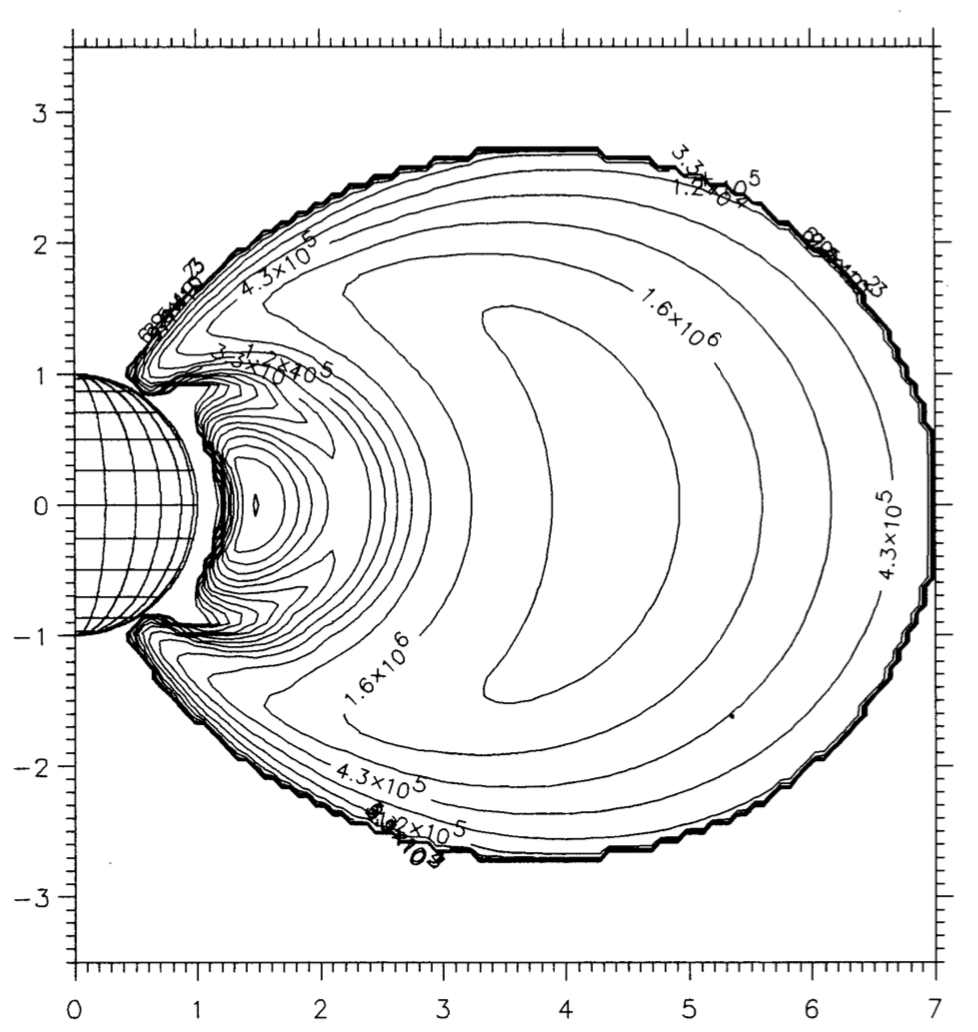
\includegraphics[scale = 0.50]{imgs/radbelt4.png}
  \caption{Electron radiation belt. \cite{bib2}}
  \label{fig:radbel4}
\end{figure}
%
\paragraph{Dynamic of the radiation Belts}

Starting from the 1990s the American satellite CRRES has shown te extreme dynamics of protons and electrons trapped in the radiation belts. In fact the population of these particles is strongly dependent on two factors:
\begin{enumerate}
    \item The Sources - injections from the tail of the magnetosphere and creations by nuclear reactions
    \item The Losses - Precipitations in the upper atmosphere or by charge exchange with particles from the Exosphere. 
\end{enumerate}

\paragraph{Dynamics on the scale of the Solar cycle-Protons}

The radiation belt of protons having high energies, more than 10 MeV varies slowly as function of the solar cycle, as shown in Fig:\ref{fig:radbel5}. The flux levels oscillates around its maximum at the minimum activity of the Sun and vice versa. This is the actual result of two different phenomena, the absorption of the protons by the upper atmosphere and the modulation of CRAND (Cosmic Ray Albedo Neutron Decay) source. This balance is shown in Fig:\ref{fig:radbel5}.



\begin{figure}[h!]
\centering
  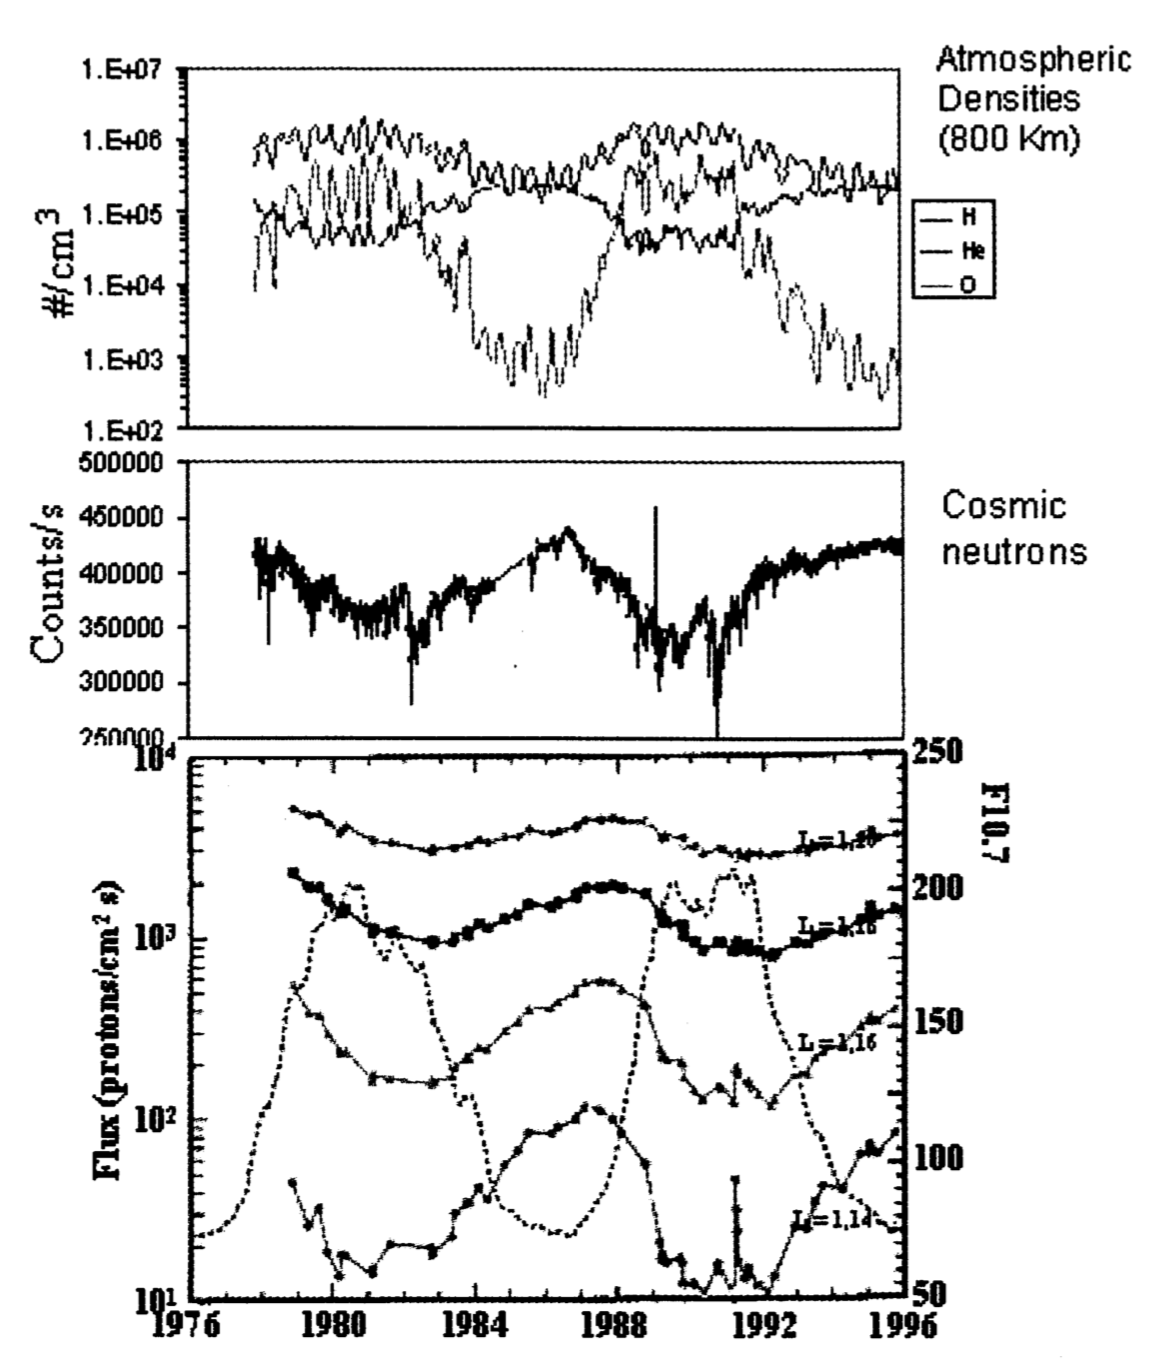
\includegraphics[scale = 0.50]{imgs/radbelt5.png}
  \caption{Changes in the proton fluxes at low altitudes (bottom), in the cosmic radiation (middle) and atmospheric densities (top) as a function of the solar cycle. \cite{bib2}}
  \label{fig:radbel5}
\end{figure}

\paragraph{Dynamics on the scale of the Solar Cycle-Electrons}
As well as for the proton cycle, the electrons, especially in the geostationary orbit, follow a similar trend. Inversely proportional to the Sun activity cycle, as shown in Fig:\ref{fig:radbel6}


\begin{figure}[h!]
\centering
  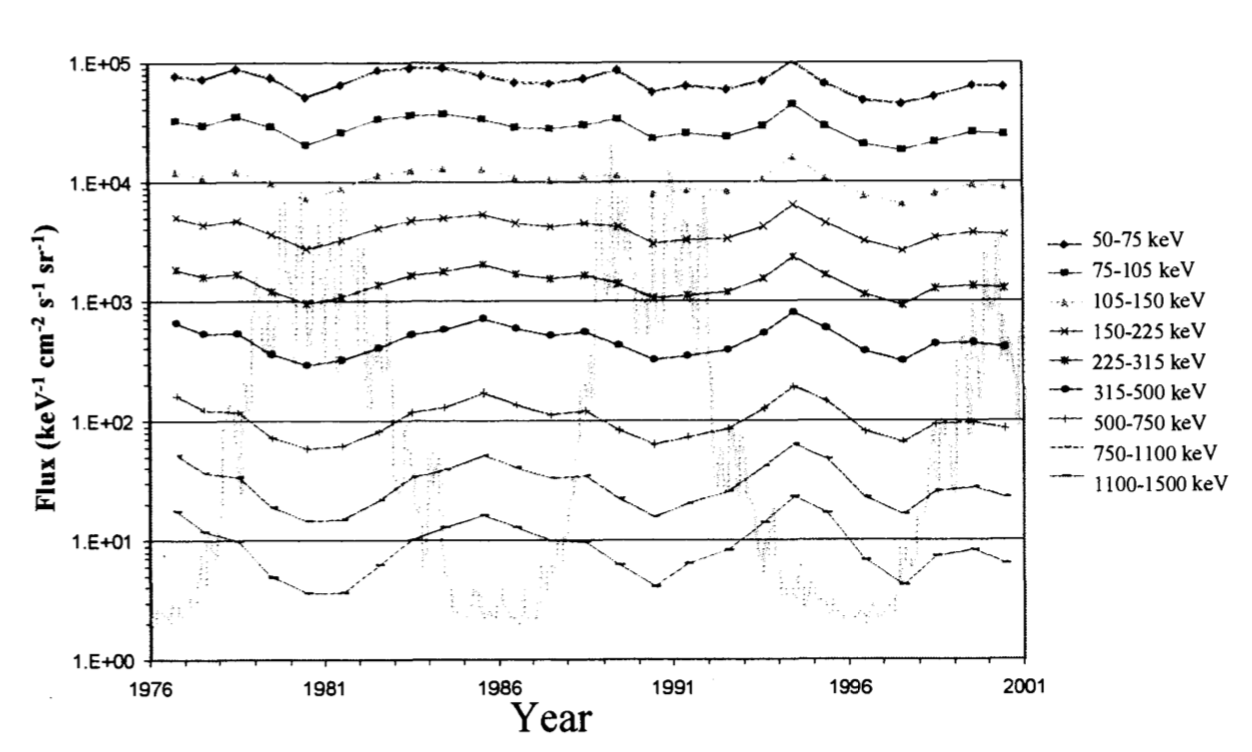
\includegraphics[scale = 0.50]{imgs/radbelt6.png}
  \caption{Electron fluxes at geostationary orbit as a function of the solar cycle. \cite{bib2}}
  \label{fig:radbel6}
\end{figure}
\iffalse

\begin{figure}[h!]
\centering
  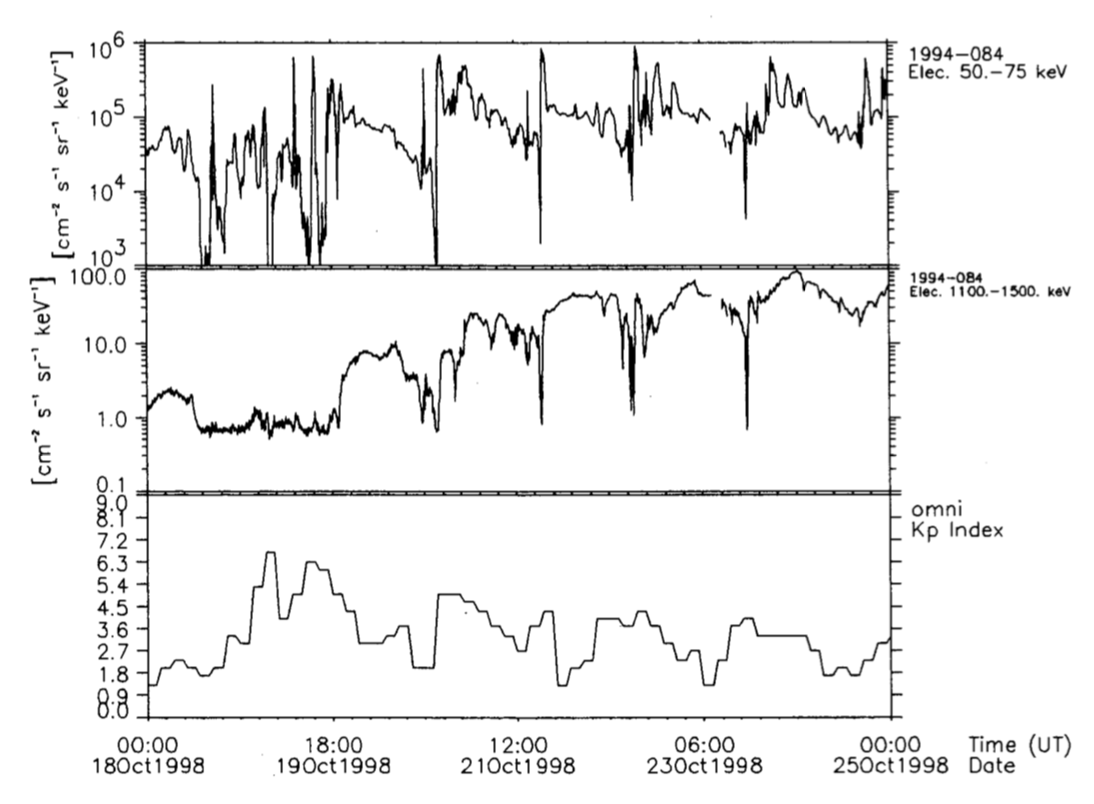
\includegraphics[scale = 0.50]{imgs/radbelt7.png}
  \caption{
Fig. 35. Flux of 50-75 keV (top), 1.1-1.5 MeV (middle) electrons in geostationary orbit and magnetic activity Kp (bottom) as a function of time (Peak intensity of the storm shown by red arrow). \cite{bib2}}
  \label{fig:radbel7}
\end{figure}

\begin{figure}[h!]
\centering
  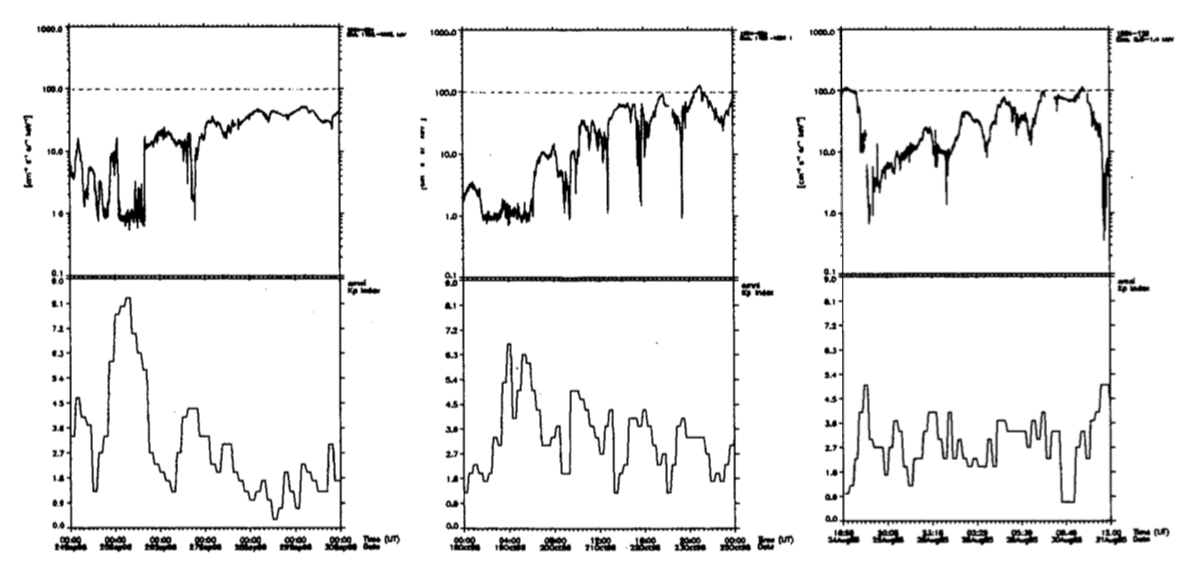
\includegraphics[scale = 0.50]{imgs/radbelt8.png}
  \caption{Comparison of the consequences of three magnetic storms on the fluxes of 1.1-1.5 MeV electrons in geostationary orbit for three different levels of activity \cite{bib2}}
  \label{fig:radbel8}
\end{figure}

\begin{figure}[h!]
\centering
  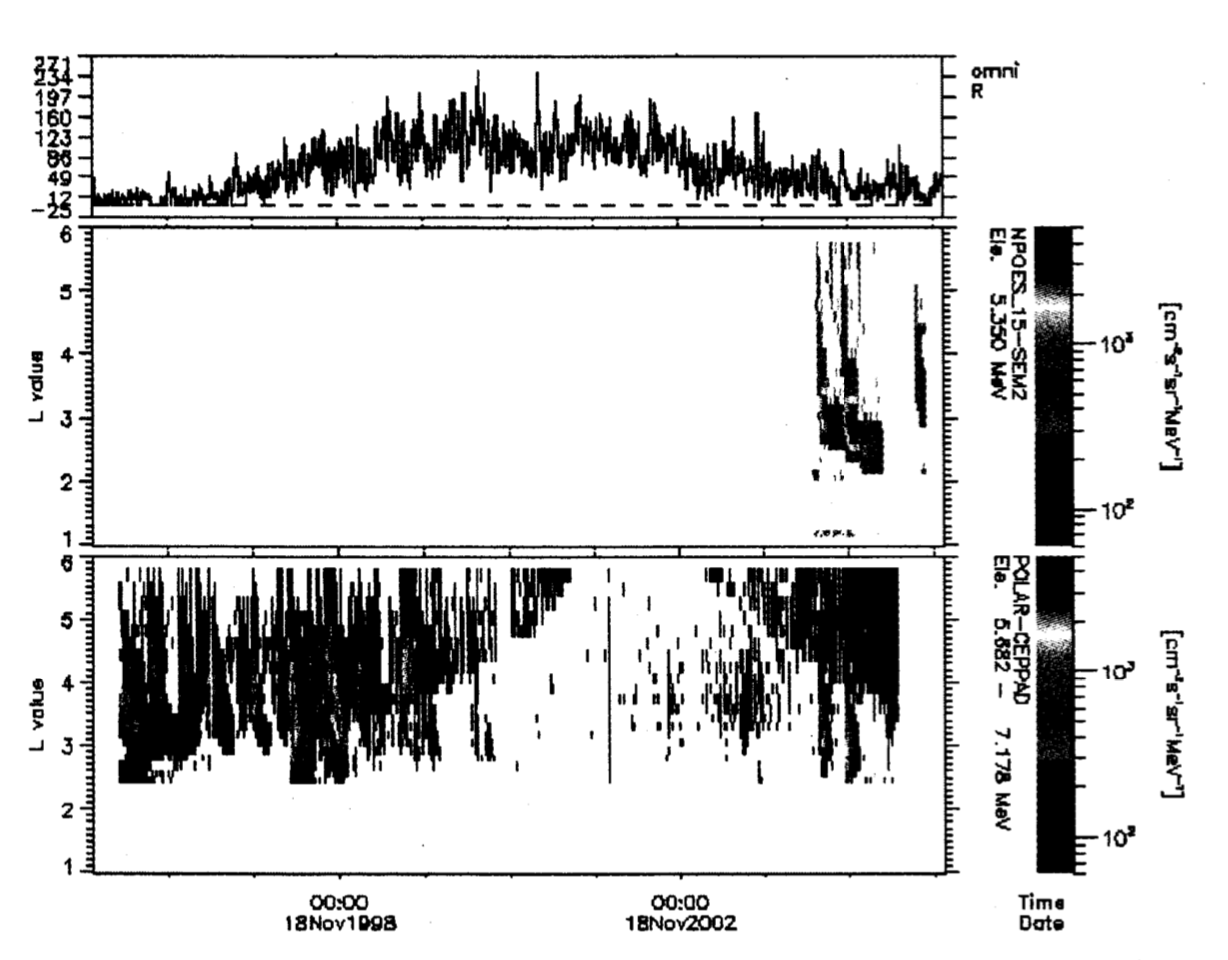
\includegraphics[scale = 0.50]{imgs/radbelt9.png}
  \caption{Top panel: Sunspot number, middle panel: 5.35 MeV electrons measured at LEO onboard NPOES-15 and bottom panel: 5.6-7.1 MeV electrons measured at H E 0 onboard Polar. \cite{bib2}}
  \label{fig:radbel9}
\end{figure}

\begin{figure}[h!]
\centering
  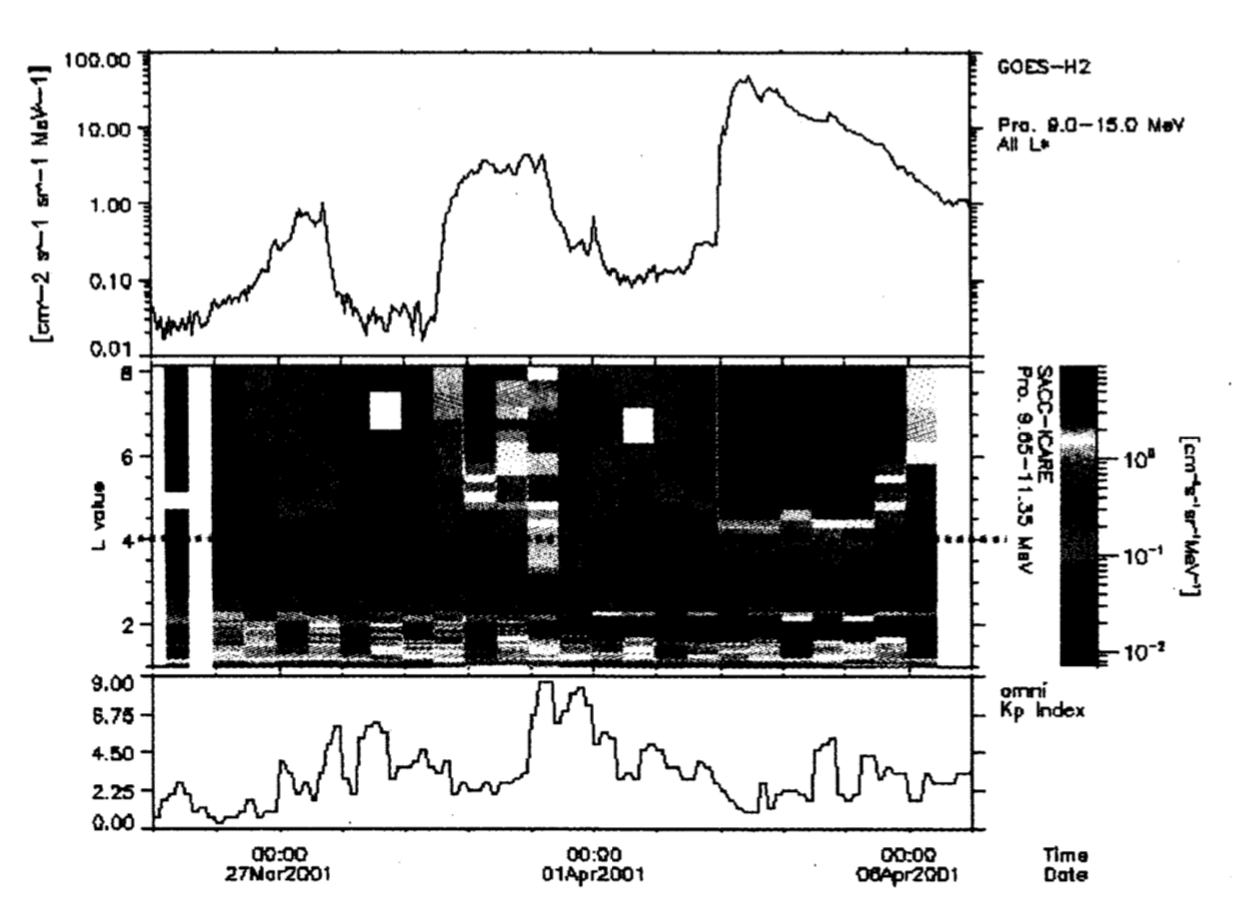
\includegraphics[scale = 0.50]{imgs/radbelt10.png}
  \caption{Top panel: Solar protons observed by GOES-8 at GEO, middle panel: 9.65-11.35 MeV protons measured at LEO onboard SAC-C and bottom panel: Kp index \cite{bib2}}
  \label{fig:radbel10}
\end{figure}

\fi

%\subsection{Solar Wind}
\newpage
\section{The Earth Environment}
Since the 1984, the existence and impact of atmospheric neutrons has been predicted. They can cause Single Event Upset in the electronics, the first actually measured was in 1992. After that several hundreds have been observed.
\begin{figure}[h!]
\centering
  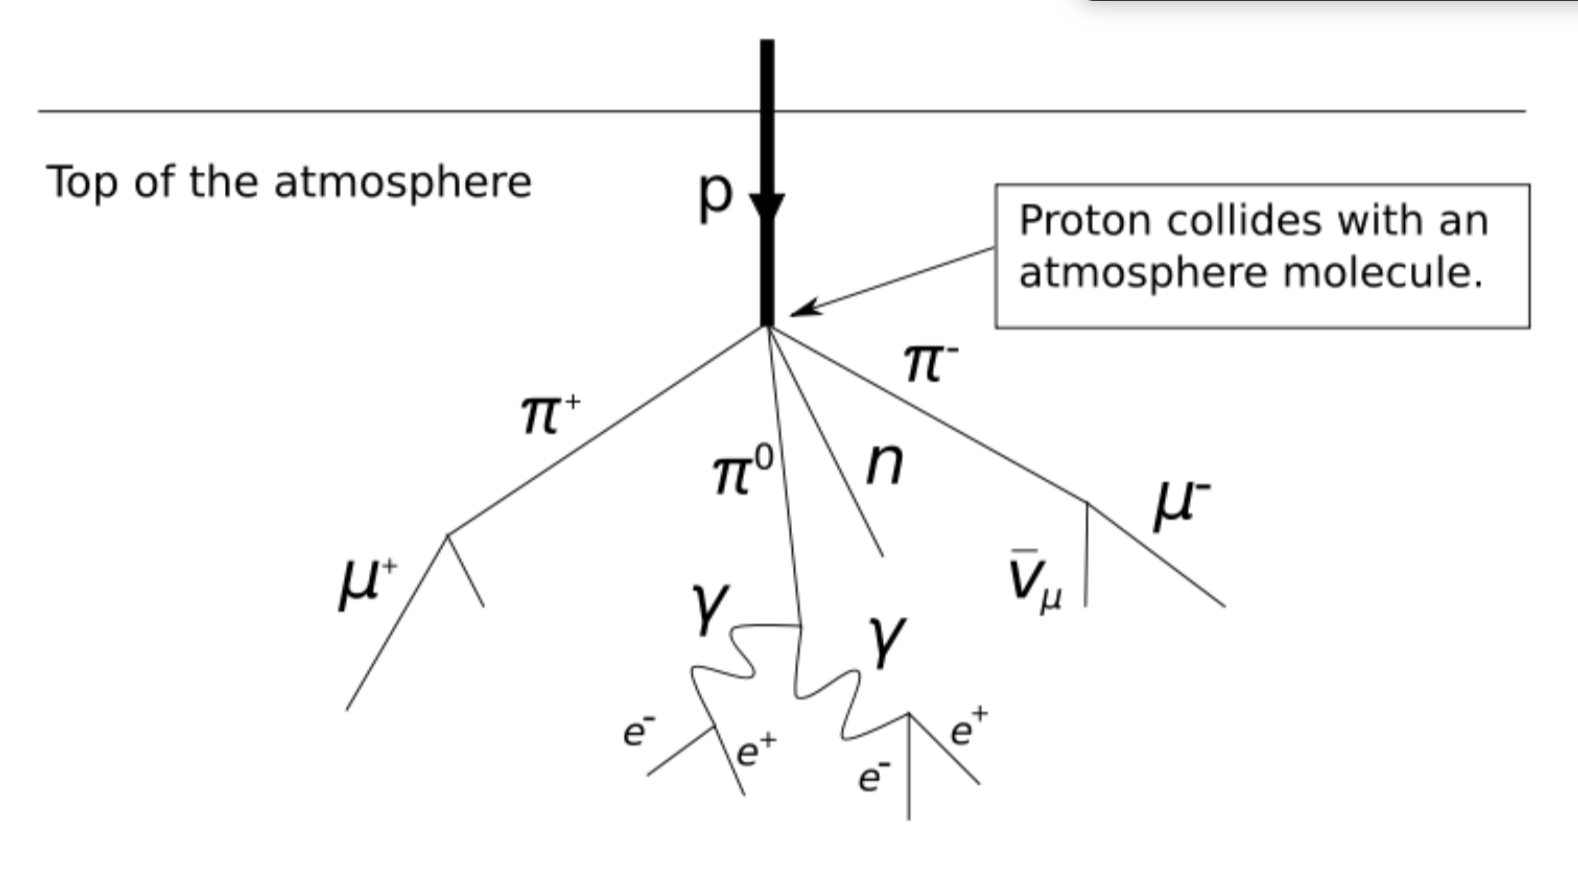
\includegraphics[scale = 0.50]{imgs/neutrons.png}
  \caption{Example of Proton Scattering \cite{bib1}}
  \label{fig:earthenv}
\end{figure}
As we can see in Fig. \ref{fig:earthenv} Cosmic rays cover a large spectrum of energies, with a comparatively high flux in the 100 MeV to 10 GeV range and a peak around 500 MeV; cosmic particles collide with the nuclei of atoms making up the Earth atmosphere and initiate the so-called air showers, producing particles such as neutrons, protons, muons, pions, electrons and gamma-rays.

A deeper analysis of the particles at commercial flight level shows a great majority of neutrons, while protons play a minor role in the Single Event Upset at those altitudes.

Moreover, even though the scheme reported in Fig. \ref{fig:earthenv} seems to be a top down shower, the neutron flux is, in fact, isotropic.


\section{Military Environment}
In case of an explosion occurring above the Earth atmosphere, two possible scenarios may be considered
\begin{itemize}
    \item Aerospace  systems  operating  at  altitudes  higher  than  50-100  km  will  be directly  submitted  to  the radiation  emitted  by  the  weapon;  hard  X-rays,  gamma-rays  and  neutrons  all  have  a  significant  impact on the electronic systems onboard satellites
    \item The main indirect effect to be considered is that related to trapping by the Earth magnetic field lines of electrons from fission debris, resulting in the formation of highly stable, artificial radiation belts which  can  deliver  much  higher  radiation  doses  to  satellites  than  natural  belts;  the  first  satellite failure  due  to  radiation  effects  dates  back  to  1963,  to  the  Starfish  test  (a  1.4  Mton  thermonuclear bomb  detonated  at  an  altitude  of  400  km);  the  test  produced  an  intense  radiation  belt  destroying  seven  satellites  over  seven  months,  primarily  because  of  dose  effects  on  their  solar  panels;  the TELSTAR satellite, launched on July 10, 1962, broke down in February 1963
\end{itemize}

A nuclear explosion in the Earth atmosphere, besides a variety of mechanical effects, is responsible for different purely radioactive effects, which can be split into two main categories 
\begin{itemize}
    \item \textbf{Initial nuclear radiation (INR)} is that released within less than a minute after detonation; X-rays are quickly stopped (at about 500 m above sea) so that gamma-rays (responsible for ionizing dose effects) and neutrons remain 
    \item \textbf{Residual nuclear radiation (RNR)} features several radiation sources; fission products, radioactivity of debris  (neutron-activated  weapon  materials),  that  of  unfissioned  uranium  and/or  plutonium  and activation of the environment; a further distinction can be made between local fallout, occurring less than  24  hours  after  explosion,  with  a  resulting  significant  level  of  ground  radiation,  and  worldwide fallout, which can take place at significant distances from the place of explosion 
\end{itemize}

\section{Radiation Effects on COTS Components}
\subsection{Basic Damage Mechanism in Semiconductor Devices}
Even if we take into consideration the great diversity of particles and their interaction with different technologies, it is possible to distinguish just two main categories of damaging mechanism for semiconductor devices
\begin{enumerate}
    \item Ionization Damage
    \item Displacement Damage
\end{enumerate}
\subsubsection{Ionization Damage}
The ionization takes place when energy deposited in a semiconductor or in insulating
layers, chiefly SiO2, frees charge carriers (electron-hole pairs), which diffuse or drift
to other locations where they may get trapped, leading to unintended concentrations
of charge and parasitic fields; this kind of damage is the primary effect of exposure
to X- and gamma-rays and charged particles; it affects mainly devices based on surface conduction (e.g. MOSFETs)\cite{bib1}. Directly ionizing radiation consists of charged
particles. Such particles include energetic electrons (sometimes called negatrons),
positrons, protons, alpha particles, charged mesons, muons and heavy ions (ionized
atoms). This type of ionizing radiation interacts with matter primarily through the
Coulomb force, repelling or attracting electrons from atoms and molecules by virtue of
their charges. Indirectly ionizing radiation consists of uncharged particles. The most
common kinds of indirectly ionizing radiation are photons above 10 keV (x rays and
gamma rays) and all neutrons. X-ray and gamma-ray photons interact with matter
and cause ionization in at least three different ways:
\begin{itemize}

\item Lower-energy photons interact mostly via the photoelectric effect, in which the
photon gives all of its energy to an electron, which then leaves the atom or
molecule. The photon disappears.
\item Intermediate-energy photons mostly interact through the Compton effect, in
which the photon and an electron essentially collide as particles. The photon
continues in a new direction with reduced energy while the released electron
goes off with the remainder of the incoming energy (less the electron's binding
energy to the atom or molecule).
\item Pair production is possible only for photons with energy in excess of 1.02 MeV.
However, near 1.02 MeV, the Compton effect still dominates: pair production
dominates at higher energies. The photon disappears and an electron-positron
pair appears in its place (this occurs only in the vicinity of a nucleus because
of conservation of momentum and energy considerations). The total kinetic
energy of the electron-positron pair is equal to the energy of the photon less the
sum of the rest-mass energies of the electron and positron (1.02 MeV). These
energetic electrons and positrons then proceed as directly ionizing radiation. As
it loses kinetic energy, a positron will eventually encounter an electron, and the
particles will annihilate each other. Two (usually) 0.511 MeV photons are then
emitted from the annihilation site at 180 degrees from each other. For a given
photon any of these can occur, except that pair production is possible only for
photons with energy greater than 1.022 MeV. The energy of the photon and the
material with which it interacts determine which interaction is the most likely
to occur\cite{bib8}.
\end{itemize}
About indirect ionization, we can say that light particles such as protons and neutrons
could have not enough LET to cause upset, but they can cause nuclear reactions that
in turn create heavier particles that can cause upsets by direct ionization. Secondary
reaction products have much higher LET but shorter ranges and lower energies\cite{bib9}.
\subsubsection{Displacement Damage}
Incident radiation dislodges atoms from their lattice site, the resulting defects altering the electronic properties of the crystal; this is the primary mechanism of device
degradation for high energy neutron irradiation, although a certain amount of atomic
displacement may be determined by charged particles (including Compton secondary
electrons); Displacement Damage mainly affects devices based on bulk conduction
(e.g. BJTs, diodes, JFETs) \cite{bib1}. Displacement damage occurs when sufficient energy
is transferred from an incident energetic particle to a lattice atom to dislodge it from
its normal location. Using Si as an example, the Si atom initially displaced by an
incoming particle is known as the primary knock-on atom (PKA) or the primary recoil.The PKA, or recoil, carries a net charge that depends on its kinetic energy.
Displacement damage occurs through the interaction of incident particles with Si
atoms by any of the following three processes:
\begin{itemize}
\item Rutherford (i.e., Coulomb) scattering
\item Nuclear elastic scattering
\item Nuclear inelastic scattering
\end{itemize}
Once any of those basic interaction processes produces a PKA, that ion subsequently
can introduce further displacement damage by Rutherford and nuclear scattering.
Lattice defects are produced by PKAs and any later-generation energetic recoils that
they create. When defects produced by incident radiation are relatively far apart,
they are known as isolated, or point, defects. As an example, isolated defects are
created by 1 MeV electrons incident on Si. Radiation-induced defects may also be
created closely together and form local regions of disorder known as defect clusters.
For example, incident 1 MeV neutrons produce both isolated and clustered defects in
Si. In general, energetic particles incident on semiconductors create either isolated
and clustered defects or solely isolated defects, depending on the mass and energy of
the incident particles. Nearly all the effects of displacement damage on the electrical and optical properties of semiconductor materials and devices can be understood
in terms of energy levels introduced in the bandgap. Those radiation-induced levels
result in the following effects: recombination lifetime and diffusion length are reduced; generation lifetime decreases; majority and minority-carrier trapping increase;
majority carrier concentration changes; thermal generation of electron-hole pairs is
enhanced in the presence of a sufficiently high electric field; tunneling at junctions
is enabled. In addition, radiation-induced defects reduce the carrier mobility and can
exhibit meta-stable configurations\cite{bib10}.

\begin{figure}[h!]
\centering
  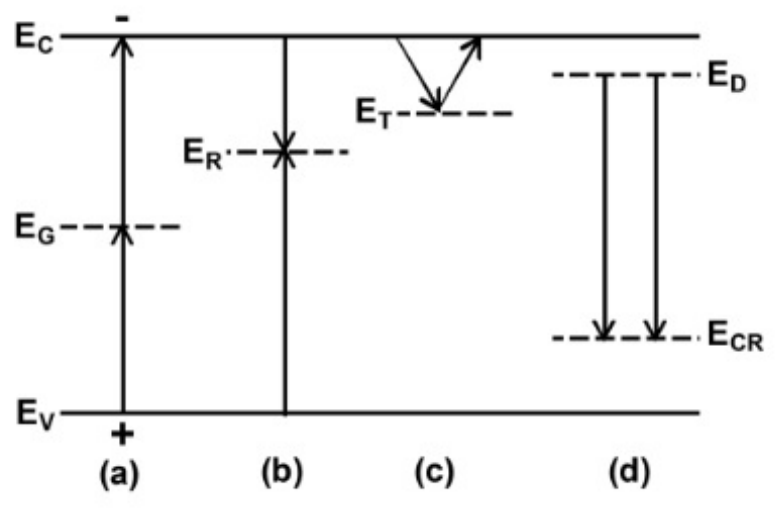
\includegraphics[scale = 0.50]{imgs/displ.png}
  \caption{Radiation-Induced energy}
  \label{fig:displ}
\end{figure}
Figure \ref{fig:displ} illustrates radiation-induced energy
levels in the Si band-gap that give rise to the following processes: (a) enhanced thermal generation; (b) enhanced recombination; (c) enhanced temporary trapping; (d)
reduced carrier concentration due, in this example, to the introduction of centers that
compensate for donors (carrier removal).
\subsection{Radiation Effects in Electronics}
As previously stated, the effects of radiation on semiconductor devices can be divided into two broad classes. Previously the Total Dose effects have been explained, now the focus will be moved to Single Event Effects.
\subsubsection{Single Event Effect}
These effects are due to the deposition of charge by a single particle that goes through a sensitive region of the device. This can lead to a destructive or non destructive damage of the device.
Moreover it is possible to identify a couple of differences between Total Dose effects and Single Event Effects:
\begin{itemize}
    \item Single Event Effects are Stochastic, while TID effects are cumulative and may occur after the device has been exposed to radiation for a long time
    \item TID are related to Long Term response, while SEE to Short term Response
    \item Only a very limited portion of the device is affected by SEE, while TID affects uniformly the entire device, this is due to the number of particles hitting the device and their distribution.
    \item While for TID the main figure is the drift of the main device parameters, concerning SEE the most important figure is the Rate of Occurrence.
\end{itemize}

We can so define this effects some of the SEE as "Soft" in case they do not induce any physical damage to the device, but just an information loss. Otherwise they are categorized as "hard" in case the impact of a heavy ion is followed by the rupture of the gate oxide. Here there is a list of the major Soft effects and Hard effects
\paragraph{Main Classes of Soft Effects}
\begin{itemize}
    \item Single Event Upset (SEU) - the corruption of a single bit in a memory array
    \item Multiple Bit Upset (MBU) - the corruption of multiple bits due to a single particle
    \item Single Event Transient (SET) - a transient signal induced by an ionizing particle in a combinatorial or analog part of a circuit
\end{itemize}
\paragraph{Main classes of hard effects}
\begin{itemize}
    \item Single Event Gate Rupture (SEGR) - rupture of gate oxide occurring especially in power MOSFETs
    \item Single Event Burnout (SEB) - burnout of a power device
    \item Single Event Latch-Up (SEL) - the activation of parasitic bipolar structures, leading to a sudden increase of the supply current
\end{itemize}

Usually in order to evaluate the occurrence of SEE the cross section of the device is used. It is defined as follow:
\begin{equation}
    \sigma_{SEE} = \frac{NumberOfEvents}{ParticleFluence}
\end{equation}

the Cross Sections varies as function of the LET of the particle hitting the device, observable only if higher than the threshold LET. The charged released by the particle hitting the transistor is collected via the so called Funneling mechanism. Most of the charge is sucked in at the struck junction through a deformation of the junction potential, while the remaining charge diffuses in the substrate and may be collected or not at the same junction\cite{bib1}

The aim of these thesis is to focus on Soft Effects, in the next section the most common SEE will be analyzed in details.
%\subsubsection{Total Ionizing Dose Effects}

\subsubsection{Radiation Effects in MOSFETs}
\paragraph{Single Event Upset}
It is obvious that in order to cause disturbance in any circuit the charge generated by a particle hitting the device must be in a sensitive node; in particular reverse biased PN junctions are the most affected by collected charge, having a larger depletion region and stronger electric field. Taking into account the case of an SRAM cell, may be the case of a particle hitting the Drain of the off NMOSFET. If that is the case the released charge is collected by the reverse-biased drain, the voltage at the struck node tends to decrease, turning the radiation-induced current in to a voltage transient. The current decreases the potential at the node, and it may go as low as below the switching voltage, changing the initial state.

These effects are function of the LET of the impinging particle and the incident angle $\theta$

\paragraph{Multiple Bit Upset}
Single events effects have become more complex  to study as the new technologies are released. In particular the minimum length that can be obtained while creating CMOS devices in lithography has gone below the micron realm. Nowadays the size of the path of the hitting particle has become comparable to the size of modern chips. Therefore that in the past may have involved a single point in the circuit now involve multiple nodes and charge sharing may occur. It follows that the rate of occurrence of Multiple Bit Upset is strongly bound to rise as fabrication process evolve.
\paragraph{Radiation Induce Latch-Up}

A latch-up is a type of short circuit which can occur in an integrated circuit. More specifically it is the inadvertent creation of a low-impedance path between the power supply rails of a MOSFET circuit, triggering a parasitic structure which disrupts proper functioning of the part, possibly even leading to its destruction due to over-current. A power cycle is required to correct this situation.

\textbf{Single event latch-up is a latch-up caused by a single event upset, typically heavy ions or protons from cosmic rays or solar flares.}
\begin{figure}[h!]
\centering
  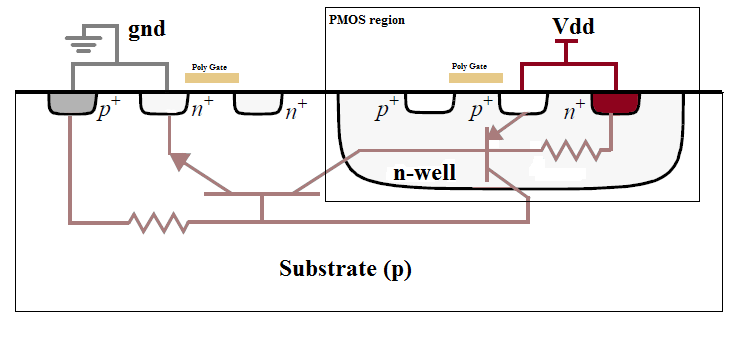
\includegraphics[scale = 0.50]{Latchup.png}
  \caption{Latch-up Diagram}
  \label{fig:coldred}
\end{figure}
The parasitic structure is usually equivalent to a thyristor (or SCR), a PNPN structure which acts as a PNP and an NPN transistor stacked next to each other. During a latch-up when one of the transistors is conducting, the other one begins conducting too. They both keep each other in saturation for as long as the structure is forward-biased and some current flows through it - which usually means until a power-down. The SCR parasitic structure is formed as a part of the totem-pole PMOS and NMOS transistor pair on the output drivers of the gates. 


\section{Types of redundant architectures}
While there are various methods to implement redundant architectures, techniques and terminologies, the following section wants to represent the most common ones used in the industry.

\subsection{Standby Redundancy}
Standby redundancy, also known as Backup Redundancy is when you have an identical secondary unit to back up the primary unit. The secondary unit typically does not monitor the system, but is there just as a spare. The standby unit is not usually kept in sync with the primary unit, so it must reconcile its input and output signals on takeover of the Device Under Control (DUC). This approach does lend itself to give a "bump" on transfer, meaning the secondary may send control signals to the DUC that are not in sync with the last control signals that came from the primary unit.
You also need a third party to be the watchdog, which monitors the system to decide when a switchover condition is met and command the system to switch control to the standby unit and a voter, which is the component that decides when to switch over and which unit is given control of the DUC. The system cost increase for this type of redundancy is usually about 2X or less depending on your software development costs. In Standby redundancy there are two basic types, Cold Standby and Hot Standby. \cite{bib12}

\subsubsection{Cold Standby Redundancy} In cold standby, the secondary unit is powered off, this is preserving the reliability of the unit. The drawback with respect to the hot standby is the longer downtime needed to switch from one unit to the secondary one. this makes it more challenging from the synchronization issues point of view.

\begin{figure}[h!]
\centering
  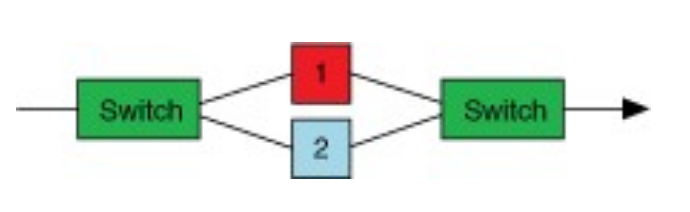
\includegraphics[scale = 0.50]{imgs/coldred.png}
  \caption{Cold Standby scheme }
  \label{fig:coldred}
\end{figure}
\subsubsection{Hot Standby Redundancy}
In hot standby instead, the secondary unit is always powered on and can eventually monitor the DUC. If the secondary unit is used as watchdog or voter to decide when to switch over, it is possible to eliminate the need for a third party unit to perform these operations. It is also possible to notice that some versions of the Hot standby are similar to the Dual Modular Redundancy (DMR) or Parallel Redundancy.

\begin{figure}[h!]
\centering
  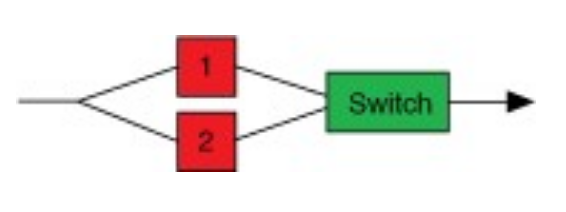
\includegraphics[scale = 0.50]{imgs/hotred.png}
  \caption{Hot Standby Schema}
  \label{fig:hotred}
\end{figure}
\subsection{N-Modular Redundancy}
N Modular Redundancy, also known as Parallel Redundancy, refers to the approach of having multiply units running in parallel. All units are highly synchronized and receive the same input information at the same time. Their output values are then compared and a voter decides which output values should be used. This model easily provides bump-less switchovers.
This model typically has faster switchover times than Hot Standby models, thus the system availability is very high, but because all the units are powered up and actively engaged with the DUC, the system is at more risk of encountering a common mode failure across all the units.

Deciding which unit is correct can be challenging if you only have two units. Sometimes you just have to choose which one you are going to trust the most and it can get complicated. If you have more than two units the problem is simpler, usually the majority wins or the two that agree win. In N Modular Redundancy, there are three main typologies: Dual Modular Redundancy, Triple Modular Redundancy, and Quadruple Redundancy.


\subsubsection{Dual Modular Redundancy}
Dual Modular Redundancy or DMR uses two identical and so functional equivalent units, both of them able to control the DUC. The most challenging side of this configuration is the switching decision between the two units. Since both of them are monitoring the DUC there is the need for a routine in case of mismatch between the two units. In is possible to create a tiebraker ore even designate the second as default winner, assuming it is more trustworty than the primary unit. 
The average cost increase of a DMR system is about twice that of a non-redundant system, factoring in the cost of the additional hardware and the extra software development time.


\begin{figure}
\centering
  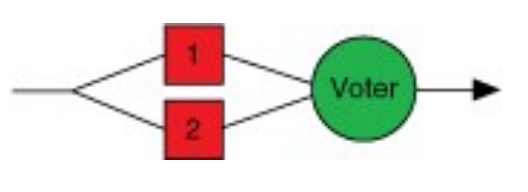
\includegraphics[scale = 0.50]{imgs/dred.png}
  \caption{DMR scheme}
  \label{fig:dred}
\end{figure}

\subsubsection{Triple Modular Redundancy}
Triple Modular Redundancy (TMR) uses three functionally equivalent units to provide redundant backup. This approach is very common in aerospace applications where the cost of failure is extremely high.

TMR is more reliable than DMR due to two main features. The most immediate is that there are two "standby" units instead of a single one. The second is that in TMR it common to see the so called diversity platforms or diversity programming techniques applied. in these techniques it is possible to notice the use of different hardware or software platforms. 

\begin{figure}[h!]
\centering
  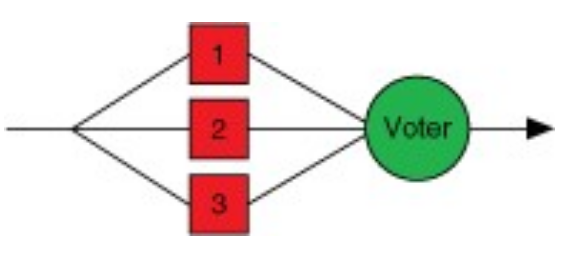
\includegraphics[scale = 0.50]{imgs/tred.png}
  \caption{TMR Schema}
  \label{fig:tred}
\end{figure}

\subsubsection{Quadruple}

Quadruple Modular Redundancy (QMR) is fundamentally similar to TMR but using four units instead of three to increase the reliability. The obvious drawback is the 4X increase in system cost.

\subsection{1:N Redundancy}

This design technique is used in case the system has a single backup for multiple modules and this backup is able to act as any of the single ones. This technique offers a redundancy at much lower costs than the others. 
This approach only works well when the primary units all have very similar functions, thus allowing the standby to back up any of the primary units if one of them fails.

Other drawbacks of this approach are the added complexity of deciding when to switch and of a switch matrix that can reroute the signals correctly and efficiently.



\begin{figure}[h!]
\centering
  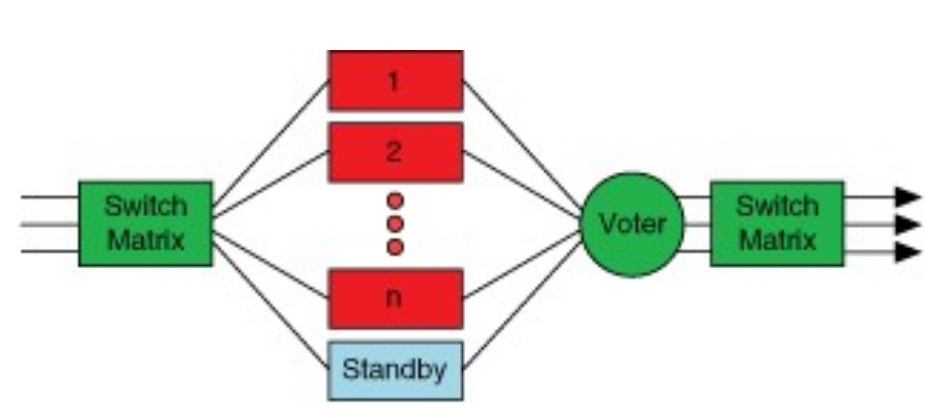
\includegraphics[scale = 0.50]{imgs/1nred.png}
  \caption{Example of Proton Scattering \cite{bib1}}
  \label{fig:1nred}
\end{figure}

\subsection{Redundancy Improves Reliability}
Reliability is defined as the probability of not failing in a particular environment for a particular mission time. Reliability is a statistical probability and there are no absolutes or guarantees. The goal is to increase the odds of success as much as you can within reason.

The following equation is the most common to calculate reliability, and it assumes that the system has a constant failure rate $\lambda$
\begin{equation}
    R(t) = e^{-\lambda t}
\end{equation}
in which:
\begin{itemize}
    \item $R(t)$ is the probability of success
    \item $t$ is the mission time or the time the system has to execute without an outage
    \item $\lambda$ is the constant failure rate over time ($N$ Failures per hour)
    \item $\frac{1}{\lambda}$ is the MTTF or mean time to failure
\end{itemize}

In fact one way  to calculate reliability is to take the probability equation and instead solve for the mean time to failure (MTTF) of the
system:

\begin{equation}
    R(t) = e^{-\lambda t } = e^{-\frac{t}{MTTF}}
\end{equation}
solving for MTTF

\begin{equation}
    MTTF = -\left( \frac{t}{\ln{[R(t)]}} \right)
\end{equation}
For example, if your application had a mission time of 24 hours a day, 7 days a week, for one year (24/7/365) and you experienced a
success rate of 90\%:
\begin{equation}
    MTTF = -\left( \frac{1yr}{\ln[.90]} \right) = 9.49 years
\end{equation}

in case redundancy has been added to the system we can, for istance, increase the success rate to 99\% for the same mission time and therefore:

\begin{equation}
    MTTF = -\left( \frac{1yr}{\ln[.99]} \right) = 99.50 years
\end{equation}
These equations effectively demonstrate the vast improvement in reliability that redundancy can bring to any system.
%\section{Open Architectures for Space Application}
\newpage
In particular, it is useful for this thesis to better understand the real advantages of TMR over the Simplex model. First we have to set some assumptions:
\begin{enumerate}
    \item TMR only works if there are at least 2 working modules
    \item $R_m$ is the Reliability of the single module
    \item $R_v$ is the Reliability of the Voter
\end{enumerate}

That said, it is possible to calculate the Reliability of a TMR system as follow:

\begin{equation}
    R_{TMR} = R_v \sum_{i=2}^{3} \binom{3}{i} R^i_m (1-R_m)^{3-i}
\end{equation}

and so 

\begin{equation}
    R_v [R_m^3 + 3R_m^2(1-R_m)] = R_v(3R^2_m - 2R_m^3)
\end{equation}

from which it is possible to evaluate the MTTF for the same system as:
\begin{equation}
MTTF_{TMR} = \int_0^{\infty}R_{TMR} dt = \int_0^{\infty}R_v (3R^2_m -2R^3_m)dt 
\end{equation}

\begin{equation}
\int_0^{\infty} e^{-\lambda_v t}\left( 3e^{-2\lambda_m t} -2e^{-3\lambda_m t}  \right) dt = \frac{3}{2\lambda_m + \lambda_v} - \frac{3}{3\lambda_m + \lambda_v}
\end{equation} 

It is possible to neglect the failure rate of the voter since it is usually designed to be way lower than the module one.

Now comparing the $MTTF_{TMR}$ with the Simplex solution we obtain:
\begin{equation}
    MTTF_{TMR} = \frac{3}{2\lambda_m} - \frac{2}{3\lambda_m} = \left( \frac{5}{6}\right) \left( \frac{1}{\lambda_m}\right) = \frac{5}{6} MTTF_{Simplex}
\end{equation}
\label{sec:iniziare}


\chapter{ISO26262}

\section{introduction}

The \textit{ISO 26262} series of standards is the adaptation of \textit{IEC 61508} series of standards to address the sector specific needs of electrical and/or electronic (E/E) systems within road vehicles. This adaptation applies to all activities during the safety limescale of safety-related systems comprised of electrical, electronic and software components. Safety is one of the key issues in the development of road vehicles. Development and integration of automotive functionalities strengthen the need for functional safety and the need to provide evidence that functional safety objectives are satisfied. With the trend of increasing technological complexity, software content and mechatronic implementation, there are increasing risks from systematic failures and random hardware failures, these being considered within the scope of functional safety. ISO 26262 series of standards includes guidance to mitigate these risks by providing appropriate requirements and processes.

To achieve functional safety, the ISO 26262 series of standards:
\begin{enumerate}
\item provides a reference for the automotive safety life cycle and supports the tailoring of the activities to be performed during the limescale phases, i.e., development, production, operation, service and decommissioning;
\item provides an automotive-specific risk-based approach to determine integrity levels [Automotive Safety Integrity Levels (ASILs)];
\item uses ASILs to specify which of the requirements of ISO 26262 are applicable to avoid unreasonable residual risk;
\item provides requirements for functional safety management, design, implementation, verification, validation and confirmation measures; and
\item provides requirements for relations between customers and suppliers.
\end{enumerate}

The ISO 26262 series of standards is concerned with functional safety of E/E systems that is achieved through safety measures including safety mechanisms. It also provides a framework within which safety-related systems based on other technologies (e.g. mechanical, hydraulic and pneumatic) can be considered. The achievement of functional safety is influenced by the development process (including such activities as requirements specification, design, implementation

The current ISO 26262 standard consists of 10 parts or phases: Vocabulary (Part 1) \cite{iso26262-1}, Management of Functional Safety (Part 2) \cite{iso26262-2}, Concept Phase (Part 3) \cite{iso26262-3}, Product Development at System Level (Part 4) \cite{iso26262-4}, Hardware Level (Part 5) \cite{iso26262-5} and Software Level (Part 6) \cite{iso26262-6}, Production and Operation (Part 7) \cite{iso26262-7}, Supporting Processes (Part 8) \cite{iso26262-8}, ASIL oriented and safety oriented analyses (Part 9) \cite{iso26262-9} and Guideline on ISO 26262 (Part 10) \cite{iso26262-10}. Based on Part 2, different phases of the product development lifecycle are assigned corresponding safety roles as shown in MISSING REF.

In order to categorize elements into Automotive Safety Integrity Levels (ASILs), it is essential to perform a comprehensive Hazard Analysis and Risk Assessment (HARA). A systematic approach involves the maintenance of a tabular record comprising all conceivable hazardous incidents. These incidents are subsequently categorized according to criteria such as: the likelihood of the event's manifestation, the extent of human intervention required to avert a potential accident upon its occurrence, and the probable gravity of the ensuing damage or harm.

Each ASIL not only establishes a methodology for error detection and management to minimize and accept residual risk, but also outlines validation procedures encompassing scrutiny and evaluation. A practical application of ISO 26262 is exemplified in \cite{westman2013reference} through the implementation of a "Fuel Level Display (FLD) system." The authors of \cite{6903180} present a safety-focused process line-oriented methodological framework, which facilitates the analysis of similarities and disparities among various safety models, thereby enablin  g the repurposing and development of an adaptable model.


\section{Overview of the standard form the Automotive point of view}

According to WHO ”1.2 million people die each year on the world's roads, with millions more sustaining serious injuries and living with long-term adverse health consequences. Globally, road traffic crashes are a leading cause of death among young people, and the main cause of death among those aged 15–29 years \cite{yeung-2018}.” Thus, road safety is a critical issue. IEC 61508 defines Safety as “the freedom from unacceptable risk of physical injury or of damage to the health of people, either directly, or indirectly as a result of damage to property or to the environment \cite{bell2006introduction}”.


\section{Main Examples of ASIL-D Chips}







\section{wWhy it may not be enough}
Standards for functional safety, such as ISO 26262 and IEC 61508, assess a system's safety based on the existence or absence of intolerable and unreasonable risk. Consequently, these standards overlook minimal acceptable risks, resulting in a lack of assurance of absolute safety. The potential for human error in risk assessment judgments, due to the nature of these standards, may have severe consequences. In \cite{7958474}, the authors explore moral concepts and challenges associated with functional safety, as well as prevalent misconceptions regarding risk perception. They utilize Kahneman's book, "Thinking, Fast and Slow" \cite{daniel2017thinking}, as the foundation for examining irrational risk judgment.

Critical ethical issues related to functional safety and risk-based decision-making processes are as follows:

\begin{itemize}
\item Diverse judgments: Variability exists among individuals' assessments of risk levels.
\item Vision Zero and Zero Tolerance: These government principles, targeting behaviors that cause harm, are not applied to functional safety.
\item Wants versus Needs: Activities such as flying and driving are human desires rather than necessities, raising questions about the justification for accommodating such desires in light of associated risks.
\item Business: The primary objective for creating safe systems should be safety, not profit, yet the pursuit of profit often drives the development of safer systems.

\end{itemize}
Additional ethical considerations encompass law, regulations, policies, evolution, innovation, and sustainability.

Addressing these issues is of paramount importance, particularly in the context of emerging autonomous systems. Current standards may be insufficient, and future work in this domain should investigate these topics further.

\end{document}
